\chapter{Evaluation and Discussion}
\label{ch:evaluation}

In this chapter we go through a few case studies and discuss the difference between the specification translations if any. Table \ref{tab:specstranslated} shows the specifications we have translated into Isabelle using \gls{zmath}. We have classified these examples to show the different types of specifications which can be translated using the \gls{zmath} toolkit. In this chapter we take one example from each class and describe in more detail how the translation was done.

\begin{table}[H]
\begin{tabular}{|l|l|}
\hline
\textbf{Examples using only terms} & \textbf{Examples using sets and terms} \\
\hline
Vending Machine & Birthday Book \\
SteamBoiler & ClubState \\
\cline{1-1}
\cline{1-1}
\textbf{Incomplete translations} & Clubstate2 \\
\cline{1-1}
Autopilot & GenDB \\
A specification which fails ZCGa & ModuleReg \\
A specification which fails ZDRa & ProjectAlloc \\
& Timetable \\
& Videoshop \\
& TelephoneDirectory \\
& ZCGa \\
\hline
\end{tabular}
\caption{A table showing the specifications we have translated into Isabelle using \gls{zmath} \label{tab:specstranslated}}
\end{table}

We have categoriesed the specification into three groups; specifications which only use terms, specifications which use both terms and set and specifications which the translation is incomplete for a variety of reasons. All the specifications we have translated are `state based specifications', which means they operate within a state and to change the state their may become precondition and postconditions within the state. Some specifications are described differently such as functional specifications, however those type of specifications are out of the scope of this thesis.

\section{Complexity of specifications}

This section we analyse the complexity of the specifications we have translate using \gls{zmath}. First we check the complexity of the raw \LaTeX{} specification file, without any annoatation. Then we discuss the complexity of the \gls{zcga} annotated specifications and \gls{zdra} annotated specifications and how this affects the translation into Isabelle.

\subsection{Raw Latex Count}

Table \ref{ch:evaluation} how long each specification is by amount of lines of code and environments uses. We have listed the specifications in decreasing complexity of how many lines of \LaTeX{} the raw specification has.

\begin{table}[H]
\centering
\begin{tabular}{|l |l | l |l |l|| l|}
\hline
\textbf{Specification} & \multicolumn{4}{l||}{\textbf{Environment}} & \textbf{Lines of \LaTeX} \\
\cline{2-5}
& Zed & Schema & Axdef & \textbf{Total} & \\
\hline
Steamboiler & 10 & 34 & 3 & 47 & 507 \\
ProjectAlloc & 4 & 17 & 0 & 21 & 213 \\
VideoShop & 3 & 15 & 0 & 18 & 166 \\
TelephoneDirectory & 6 & 11 & 0 & 17& 133 \\
ClubState & 4 & 11 & 1 & 16 &129 \\
ZCGa & 2 & 9 & 0 & 11 & 128 \\
GenDB & 2 & 7 & 0 & 9 & 114 \\
Timetable & 1 & 6 & 1 & 8 & 92 \\
BirthdayBook & 3 & 7 & 0 & 10 & 83 \\
AutoPilot & 2 & 3 & 0 & 5 & 83 \\
ClubState2 & 1 & 6 & 1 & 8 & 80 \\
Vending Machine & 4 & 7 & 0 & 11 & 68 \\
ModuleReg & 1 & 3 & 0 & 4 & 43 \\
\hline
\end{tabular}
\caption{How many zed, schema and axdef environments and lines of \LaTeX{} code makes up each specification \label{tab:numbersspec}}
\end{table}

We list information about how many different envronments and lines of \LaTeX{} make up each specification in table \ref{tab:numbersspec}. The environment numbers count how many different types of environments exist within the specification. That is how many `\verb|\begin{schema}...\end{schema}|' or `\verb|\begin{zed}|... etc. We add up the total amount of environments in the specification. From the table we can see that for most of the specifications the more lines of \LaTeX{} there is then the total amount of environments increse. However, there are three exceptions to this trend. The `\emph{BirthdayBook}' specification, `\emph{ClubState2}' specification and `\emph{Vendine Machine}' specification. Specifications for systems are can always be written in a variety of ways and still have the same meaning. Even formal specifications can be written different ways. For example one may have the following declarations:

\begin{zed}
t:\nat \\
l: \nat 
\end{zed}

However, this declaration can also be written as the following:
\begin{zed}
t,l: ;\nat
\end{zed}

Thus removing a line. Formal specifications can also include comments written in natural language which are not part of the formal script. These extra comments about the specification may have also added to the line count in table \ref{tab:numbersspec}.

\subsection{ZCGa Count}

In this section, we evaluate the \gls{zcga} annotations on the specifications. We describe how many of each \gls{zcga} annotations occurs for each specification we have translated.

\begin{table}[H]
\centering
\begin{tabular}{|l |l | l |l | l| l | l |}
\hline
\textbf{Specification} & \multicolumn{6}{c|}{\textbf{ZCGa WeakTypes}}\\
\cline{2-7}
 & \cgatext{} & \declaration{} & \expression{} & \term{} & \set{} & \definition{} \\
\hline
Steamboiler & 297 & 26 & 282 & 595 & 4 & 0 \\
ProjectAlloc & 98 & 43 & 113 & 154 & 165 & 0\\
VideoShop  & 87 & 31 & 75 & 119 & 95 & 0 \\
TelephoneDirectory & 78 & 26 & 53 & 72 & 50 & 0 \\
ClubState & 75 & 17 & 51 & 55 & 51 & 0 \\
ZCGa & 73 & 27 & 67 & 35 & 133 & 0 \\
GenDB & 45 & 24 & 71 & 117 & 121 & 1 \\
Timetable & 35 & 15 & 53 & 48 & 114 & 0 \\
BirthdayBook & 26 & 11 & 24 & 28 & 19 & 0 \\
AutoPilot & 16 & 9 & 19 & 31 & 2 & 0\\
ClubState2 & 34 & 7 & 37 & 22 & 72 & 0 \\
Vending Machine & 16 & 7 & 21 & 37 & 0 & 0 \\
ModuleReg & 20 & 6 & 18 & 13 & 31 & 0 \\
\hline
\end{tabular}
\caption{How many of each grammatical category exists in each specification. \label{tab:specgram}}
\end{table}

The amount of times a \gls{zcga} weak type occurs in each specification is shown in table \ref{tab:specgram}. We remind the reader the colours corresponding to each grammatical type are: \cgatext{schematext}, \declaration{declaration}, \expression{expression}, \term{term}, \set{set} and \definition{definition}. In this instance we don't use \specification{specification} as we assume each document contains a single specification.

In our sample set we only have one specification (GenDB) with a `\texttt{definition}' annotation. This \texttt{definition} is locally defined within the specification. The `\emph{Vending Machine}' specification only uses \texttt{terms} and therefore there are no \gls{zcga} \texttt{term} annotations. However the `\emph{StemBoiler}' specification also only uses term yet there are 4 \texttt{set} \gls{zcga} annotations. This is because some of the \texttt{terms} used in the specification have to be intrduced by a \texttt{set}. For example in the \emph{SteamBoiler} specification we have the following annotation:

\begin{verbatim}
\begin{zed}
\set{State} ::= \term{init} | \term{norm} |
\term{broken} | \term{stop}
\end{zed}
\end{verbatim}

Although the set \verb|State| is annotated as a set, it is not used in any of the schema's in the rest of the specification. It is only defined to present the terms \verb|init|, \verb|norm|, \verb|broken| and \verb|stop| which are used in the specification.

We expect there to be more \texttt{schemaText}'s then \texttt{declarations} and \texttt{expressions} combined as \texttt{schemaText} contains all \texttt{declarations}, \texttt{expressions} and SchemaNames however, from the table we can see that this is not always the case. For example in the \emph{ProjectAlloc} example, there are 98 \texttt{schemaText}, 43 \texttt{declarations} and 113 \texttt{expressions}. The reason for this could be because a single \texttt{expression} can in itself contain many \texttt{expressions}. For example the following \texttt{schemaText} has been taken from the \emph{ProjectAlloc} specification:

\begin{verbatim}
\text{\expression{\forall 
\declaration{\term{lec}: \expression{\dom maxPlaces}}\\
@ \expression{\term{\# (\set{\set{allocation}
\rres \set{\{\term{lec}\}}})} \leq \term{\set{maxPlaces}~\term{lec}}}}}
\end{verbatim}

In this example we can see that there contains 1 annotated \texttt{schemaText} but 3 \texttt{expressions}.
Another reason why there may be more \texttt{expressions} than \texttt{schemaText} is because when annotating a specification with \gls{zcga}, \texttt{declarations} also contain \texttt{expressions}. If we have the following example, again taken from the ProjectAlloc specification:

\begin{verbatim}
\text{\declaration{\set{studInterests}, \set{lecInterests}:
\expression{PERSON \pfun\iseq TOPIC}}}
\end{verbatim}

The \gls{zcga} text contains 1 annotation of \texttt{SchemaText}, 1 annotation of a \texttt{declaration}, 2 annotations of \texttt{sets} and 1 annotation of an \texttt{expression}. Since this is the case we expect to see more expressions than declarations in every specification, which is true according to table \ref{tab:specgram}.


\subsection{ZDRa Count}

In this section we analyse the amount of \gls{zdra} instances and relations are labeled for each of the specifications we translated. We give details of the amount of instances in table \ref{tab:speczdracount} and give details of the amount of relations in each specification in table \ref{tab:speczdrarelationscount}.

\begin{table}[H]
\centering
\begin{tabular}{|l |l | l |l | l| l | l | l | l | l | l |}
\hline
\textbf{Specification} & \multicolumn{10}{c|}{\textbf{ZDRa Instances}}\\
\cline{2-11}
 & \textbf{A} & \textbf{SS} & \textbf{IS} & \textbf{CS} & \textbf{OS} & \textbf{TS} & \textbf{PRE} & \textbf{PO} & \textbf{O} & \textbf{SI}  \\
\hline
Steamboiler & 6 & 2 & 2 & 21 & 6 & 6 & 21 & 23 & 12 & 1  \\
ProjectAlloc & 0 & 1 & 1 & 5 & 11 & 0 & 11 & 6 & 22 & 1 \\
VideoShop &  0 & 1 & 1 & 3 & 10 & 0 & 13 & 4 & 20 & 1  \\
TelephoneDirectory & 0 & 1 & 1 & 4 & 5 & 5 & 8 & 5 & 10 & 1 \\
ClubState & 1 & 1 & 1 & 4 & 6 & 4 & 9 & 6 & 11 & 0 \\
ZCGa & 0 & 1 & 1 & 6 & 1 & 0 & 6 & 7 & 2 & 1 \\
GenDB & 0 & 1 & 1 & 4 & 2 & 0 & 6 & 5 & 4 & 1 \\
Timetable & 1 & 1 & 1 & 4 & 0 & 0 & 4 & 5 & 0 & 1 \\
BirthdayBook & 0 & 1 & 1 & 1 & 4 & 2 & 4 & 2 & 8 & 1 \\
AutoPilot & 0 & 2 & 0 & 1 & 1 & 0 & 1 & 1 & 2 & 0 \\
ClubState2 & 1 & 2 & 1 & 3 & 0 & 0 & 3 & 4 & 0 & 2 \\
Vending Machine & 0 & 1 & 0 & 3 & 0 & 3 & 3 & 2 & 0 & 0 \\
ModuleReg & 0 & 1 & 0 & 2 & 0 & 0 & 2 & 2 & 0 & 1 \\
\hline
\end{tabular}
\caption{How many of each ZDRa instances exists in each specification. \label{tab:speczdracount}}
\end{table}

From table \ref{tab:speczdracount} we can see that all specifications have either 1 or 2 statesSchema's. For state base specification it should be the case that then specification has at least 1 state. Most state based specifications have stateInvariants that must be conformed to through all the changes of the specification. However this is not a must and some specification (even from our sample) do not have any stateInvariants. 

All precondition must have a corresponding postcondition or output, therefore we can say:

\begin{lemma}
$precondition \longrightarrow postcondition \lor output$
\end{lemma}

The table supports this informatio as there are more combined postconditions and outputs then there are precondition. However not all postconditions and outputs need to have a precondition, they can be executed without one. Therefore the number of preconditions does not need to equal the total number of postcondition and outputs.

\begin{table}[H]
\begin{tabular}{|l |l | l |l | l| l |}
\hline
\textbf{Specification} & \multicolumn{5}{c|}{\textbf{ZDRa Relations}}\\
\cline{2-6}
 & \textbf{initiaOf} & \textbf{requires} & \textbf{allows} & \textbf{totalises} & \textbf{uses} \\
\hline
Steamboiler & 2 & 28 & 21 & 24 & 92  \\
ProjectAlloc & 1 & 16 & 11 & 0 & 16  \\
VideoShop  & 0 & 15 & 13 & 0 & 142  \\
TelephoneDirectory &  1 & 11 & 8 & 14 & 8 \\
ClubState &  1 & 12 & 9 & 14 & 12  \\
ZCGa & 1 & 9 & 6 & 0 & 7  \\
GenDB & 1 & 8 & 6 & 0 & 6  \\
Timetable & 1 & 6 & 4 & 0 & 6  \\
BirthdayBook & 1 & 7 & 4 & 6 & 5  \\
AutoPilot & 0 & 2 & 1 & 0 & 2 \\
ClubState2 & 1 & 6 & 3 & 0 & 6 \\
Vending Machine & 0 & 2 & 0 & 2 & 8  \\
ModuleReg & 0 & 3 & 2 & 0 & 2  \\
\hline
\end{tabular}
\caption{How many of each ZDRa relations exists in each specification. \label{tab:speczdrarelationscount}}
\end{table}

We can cross reference the table showing the amount of instances (table \ref{tab:speczdracount}) with the table showing the relations (table \ref{tab:speczdrarelationscount}). For example, the relation \emph{initialOf} can only occur if the specification has an \emph{initialSchema}. Not all specifictions have an \emph{initialSchema} and therefore do not have an \emph{initialOf} relation.

There is also an equal amount of \emph{allows} relations as there is \emph{preconditions}. As was written previously, all preconditions must have a corresponding output or postcondition, therefore the relation `\emph{allows}' links each precondition to its corresponding postcondition or output. However, the vendingMachine specification is an exception to this as the preconditions are written as entire schema's. For example we have the following instance in the vending machine specification:

\begin{verbatim}
\draschema{PRE3}{
\begin{schema}{some\_stock}
stock: \nat
\where
stock > 0
\end{schema}}
\end{verbatim}

This chunk of specification describes an entire schema as a precondition. The totalising schema then joints the precondition to their corresponding output or postcondition. The specification is written in this way as it is a personal choice of writing the specification formally. All other specifications in our sample set are written in the style where the precondition and corresponding output or postcondition are written inside the same schema environment.

Obviously, the relation `\emph{totalises}' only occurs in specifications where totaliseSchema's are present. Therefore the `\emph{totalise}' relation is not necessary in all specifications.

VideoShop specification is one of the largest specifications (in terms of lines of \LaTeX{}) in our sample set however it has quite a small amount of relations.

\section{Case Studies}

This section describes a few specification case studies in which we have used the \gls{zmath} tool kit to translate and prove formal specifications into the Isabelle automated theorem prover. The first case study present a formal specification only using terms, the second is a formal specification where both sets and terms are used and therefore the syntax used in Isabelle is more complex. The final case study we present is a partial translation of a specification which is not fully formalised but on it's way to becoming fully formal.

\subsection{Case Study 1: A specification using only terms.}
\label{subsec:casestudy1}

The following case study is based on the \emph{Steamboiler} \cite{steamboilerslides} specification which has been translated and proved in Isabelle using the \gls{zmath} framework. This case study only uses variables which are terms. The steamboiler specification is the larges from our examples. It is made up of 507 lines of \LaTeX{} code, 10 zed environemnts, 34 schmes and 3 axiom definitions. When annotating with \gls{zcga} there were 297 schematext, 26 declarations, 282 expressions, 595 terms and 4 sets. When annotated with \gls{zdra} there were 6 axioms, 2 stateSchema's, 2 initialSchema's, 21 changeSchema's, 6 outputSchema's, 6 totaliseSchema's, 21 preconditions, 23 postconditions, 12 outputs and 1 set of stateInvariants.

\subsubsection{Natural Lanaguge Specification of the Steamboiler}

The steam boiler itself is a water level and steam quantity measuring device, with four pumps and four pump controlers. There is a valve for emptying the boiler.

\begin{figure}[H]
\centering
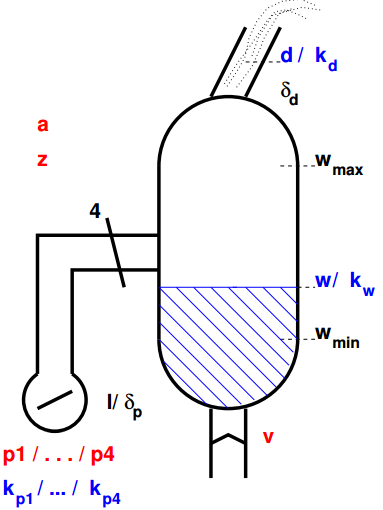
\includegraphics[scale=0.5]{Figures/Evaluation/steamboilerimage.png}
\caption{A diagram showing a theoretical Steamboiler. \label{fig:steamboiler}}
\end{figure}

An example of how the steamboiler could look is shown in figure \ref{fig:steamboiler}. The variables of the steamboiler are shown in table \ref{tab:steamboilervariables}.

\todo[inline]{find out what $l$ does}
\begin{table}[H]
\begin{tabular}{l|l}
\textbf{variables} & \textbf{description} \\
\hline
$w_{min}$ & minimal water level \\
$w_{max}$ & maximal water level \\
$l$ & \\
$d_{max}$ & maximal quantity of steam exiting the boiler \\
$\delta_{p}$ & error in the value of the pumps \\
$\delta_{d}$ & error in steam\\
$w$ & water level \\
$d$ &  amount of steam exiting the boiler \\
$k_{p,i}$ & pump $i$ works/broken \\
$k_{w}$ & water level measuring device works/broken \\
$k_{d}$ & steam amount measuring device works/broken\\
$p_{i}$ & pump $i$ on/off \\
$v$ & valve open/closed \\
$a$ & boiler on/off \\
$z$ & state init/norm/broken/stop 
\end{tabular}
\caption{The variables of the steamboiler and their descriptions. \label{tab:steamboilervariables}}
\end{table}

The full formal specification for the steamboiler is 10 pages long which can be found in \cite{mathlangexamples}. Therefore we have given small examples taken from the full specification.

\subsubsection{ZMathLang steps for the steamboiler case study.}

\begin{figure}[H]
\centering
\begin{minipage}{0.45\textwidth}
\centering
\includegraphics[scale=0.6]{{Figures/Evaluation}/0steamboilerimage.png}
\vspace{-0.18in}
\caption{The formal specification \LaTeX{} code for the steamboiler system. \label{fig:steamboiler0}}
\vspace{-0.2in}
\end{minipage}\hfill
\begin{minipage}{0.45\textwidth}
\centering
%[clip,l,b,r,t]
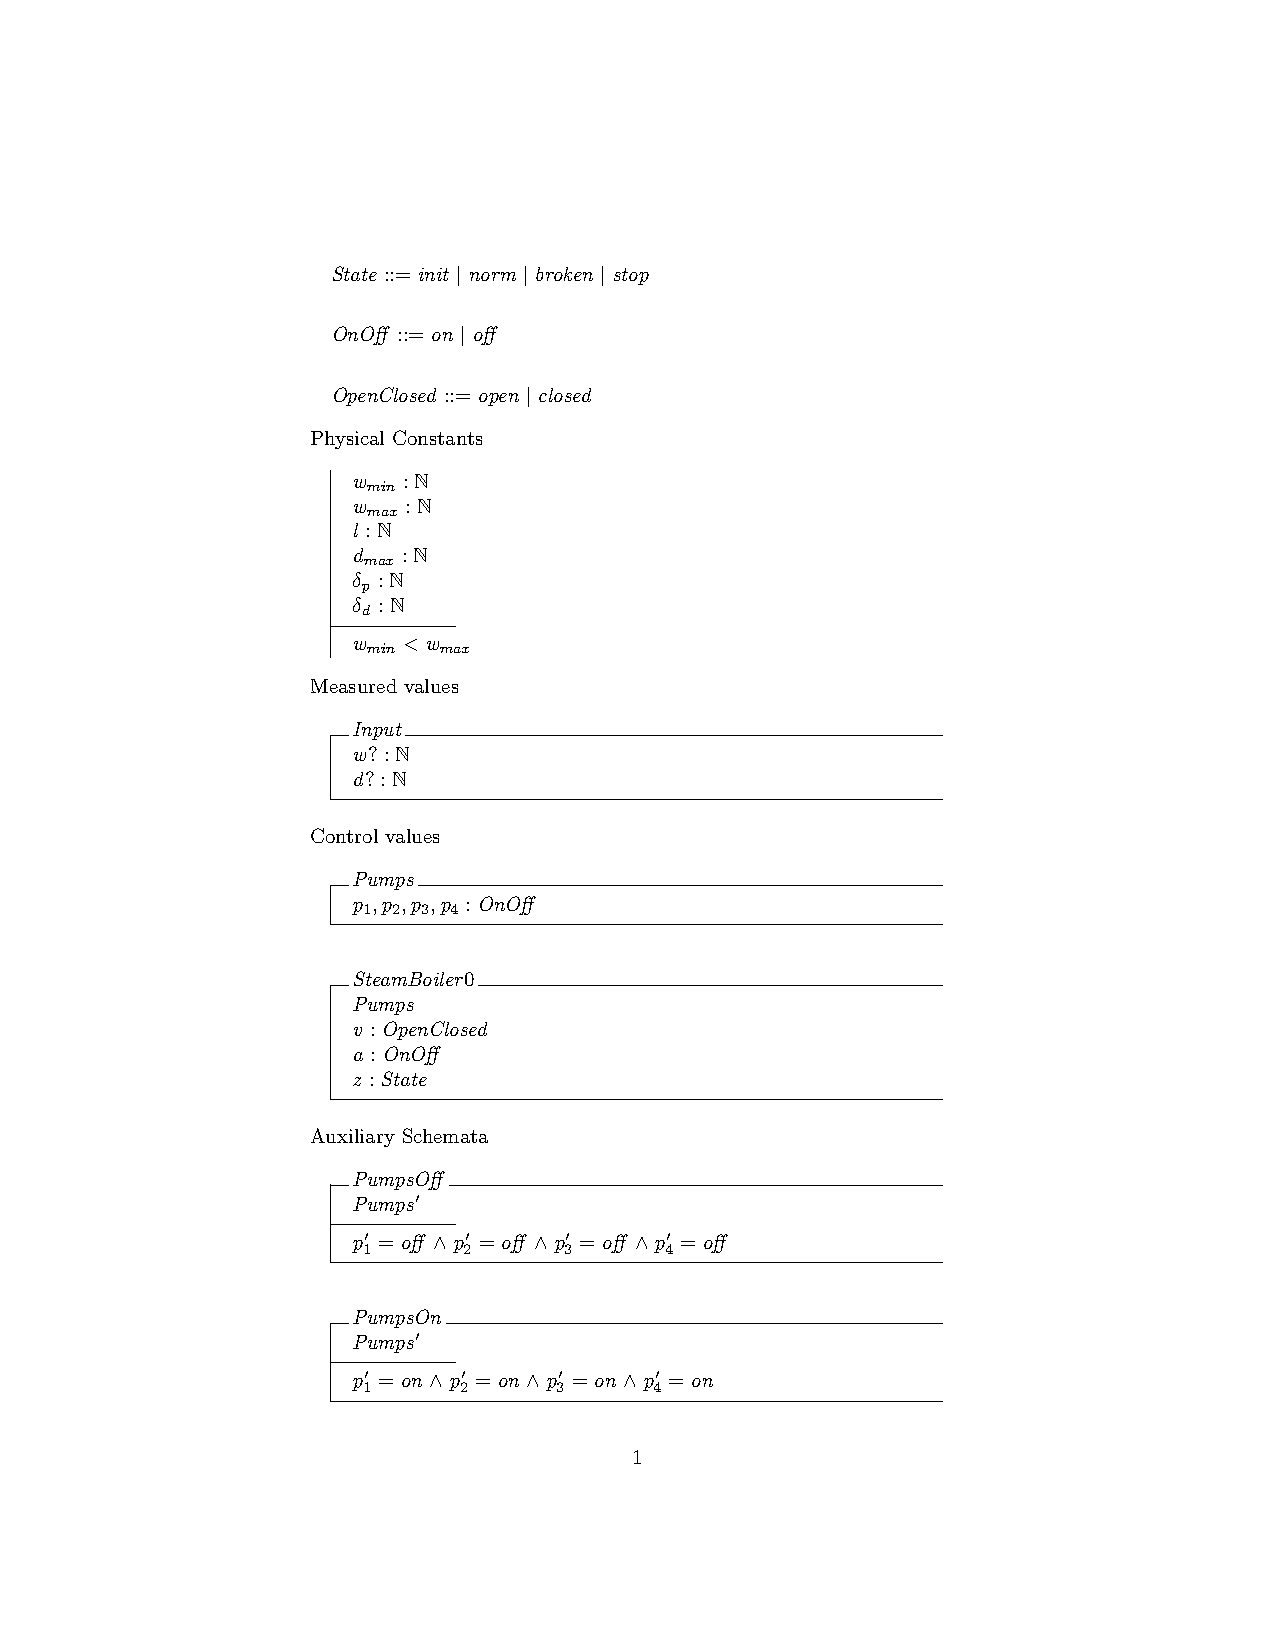
\includegraphics[clip, trim=5.5cm 4cm 5cm 4cm, scale=0.6]{examples/steamboiler/0.pdf}
\vspace{-0.2in}
\caption{The formal specification for the steamboiler system. \label{fig:steamboiler0comp}}
\vspace{-0.2in}
\end{minipage}
\end{figure}

We show the \LaTeX{} code for part of the raw steamboiler specification in figure \ref{fig:steamboiler0} and it's pdflatex counterpart in figure \ref{fig:steamboiler0comp}.

We then annotate the specification using \gls{zcga} and \gls{zdra} labels.

\begin{figure}[H]
\centering
\begin{minipage}{0.45\textwidth}
\centering
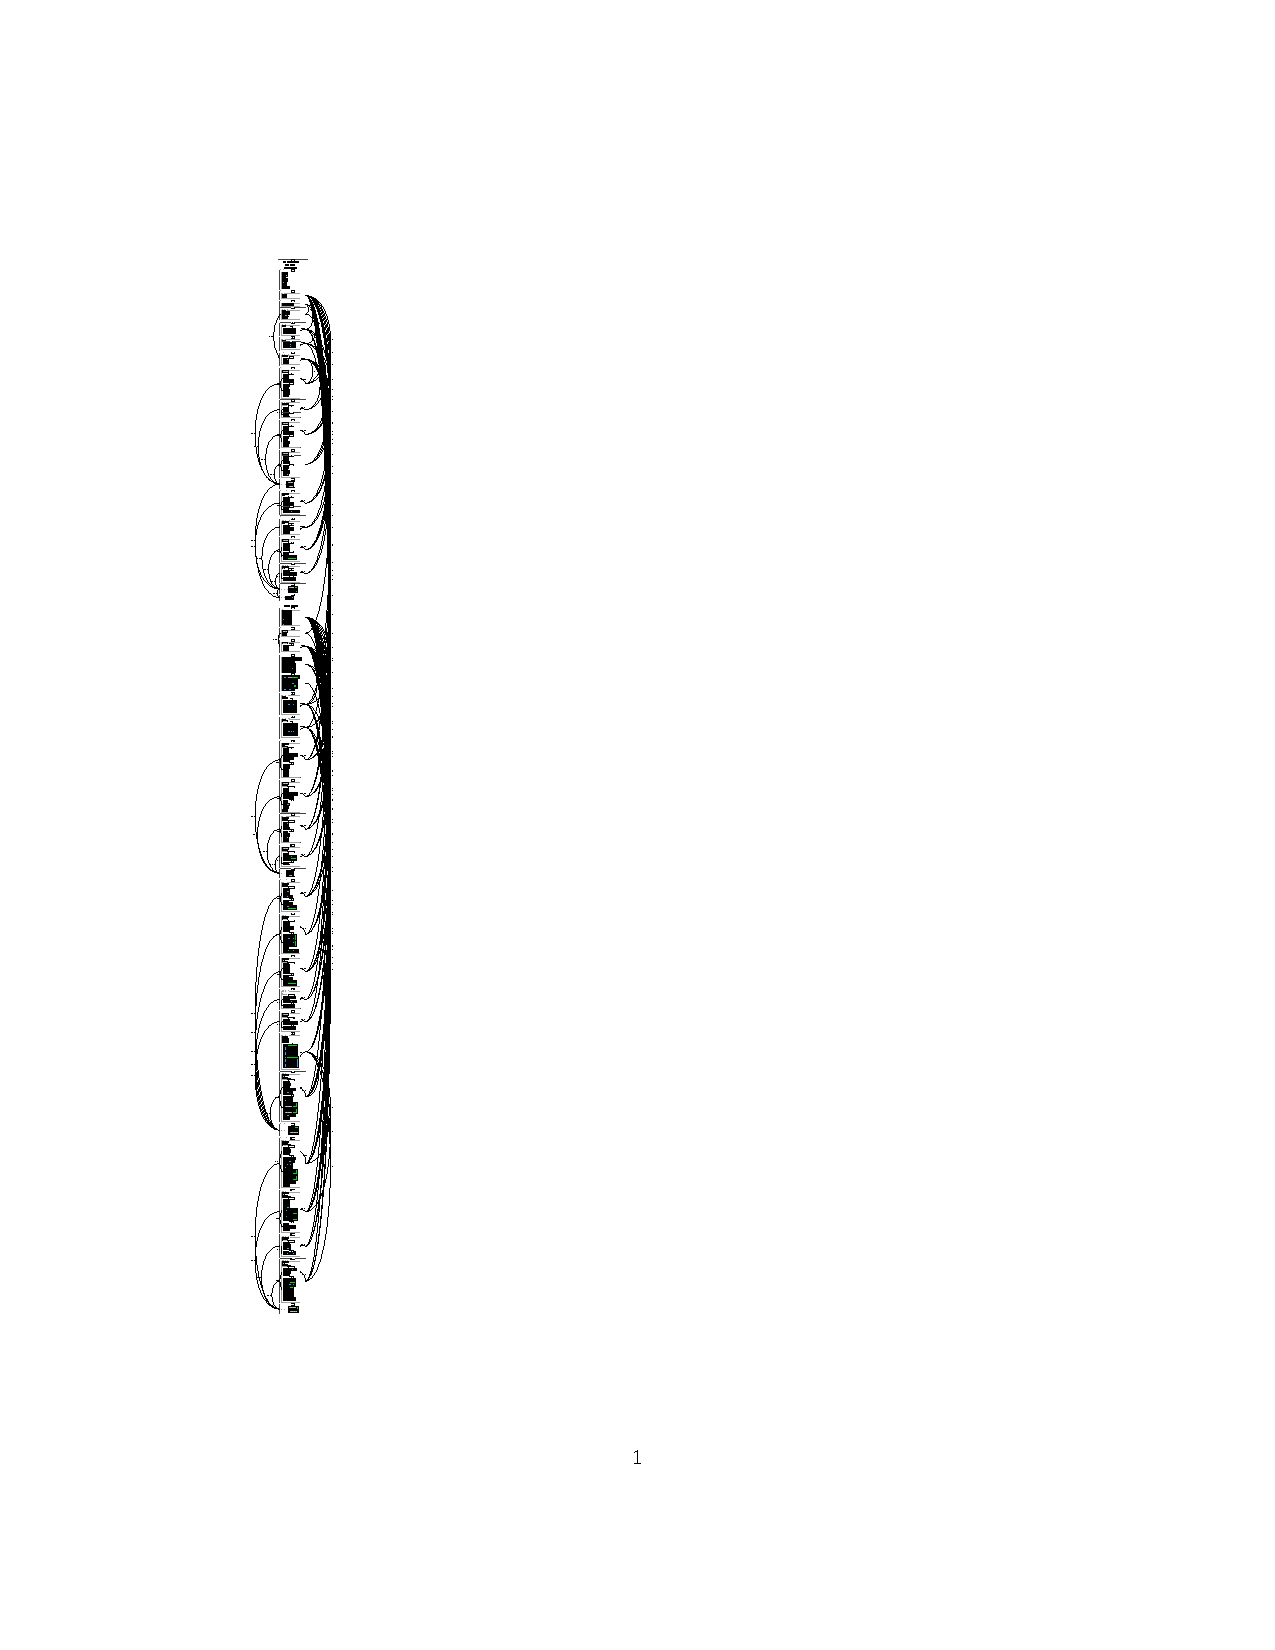
\includegraphics[clip, trim=3cm 8cm 6cm 2cm]{examples/steamboiler/1n2.pdf}
\vspace{-0.18in}
\caption{An example of the original steamboiler specification annotated in \gls{zcga} and \gls{zdra}. \label{fig:steamboilert1n2}}
\vspace{-0.2in}
\end{minipage}\hfill
\begin{minipage}{0.45\textwidth}
\centering
%[clip,l,b,r,t]
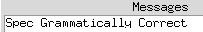
\includegraphics[ scale=0.5]{examples/steamboiler/zcgacorrect.png}
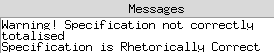
\includegraphics[ scale=0.5]{examples/steamboiler/zdracorrect.png}
\vspace{-0.2in}
\caption{The outputting result when checking the steamboiler specification with the \gls{zcga} and \gls{zdra} checkers. \label{fig:steamboilercorrect}}
\vspace{-0.2in}
\end{minipage}
\end{figure}

Since we only have a warning and no errors when checking the steamboiler specification we can now generate a goto graph and dependency graphs for it.

\begin{figure}[H]
\centering
\begin{minipage}{0.45\textwidth}
\centering
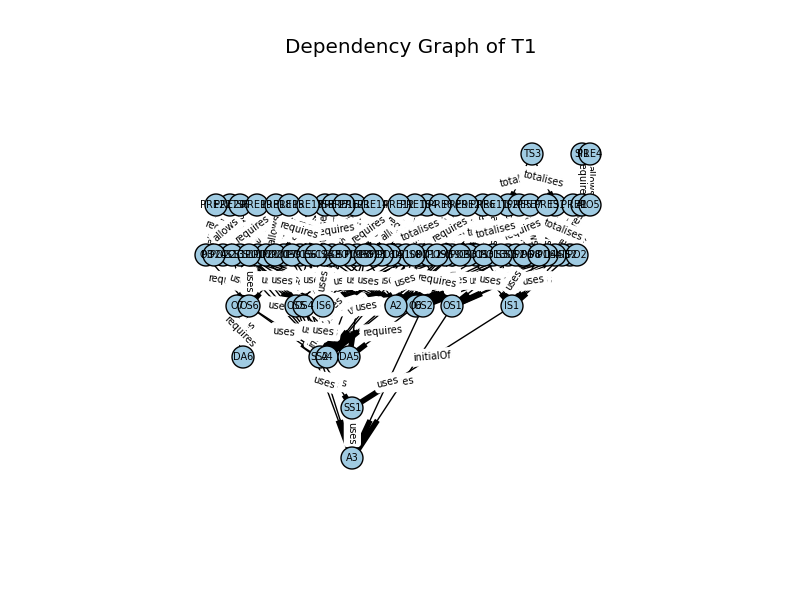
\includegraphics[trim=4cm 1cm 1cm 1cm, scale=0.5]{examples/steamboiler/25a.png}
\vspace{-0.18in}
\caption{The dependecy graph produced for the steamboiler specification. \label{fig:steamdepgraph}}
\vspace{-0.2in}
\end{minipage}\hfill
\begin{minipage}{0.43\textwidth}
%[clip,l,b,r,t]
\centering
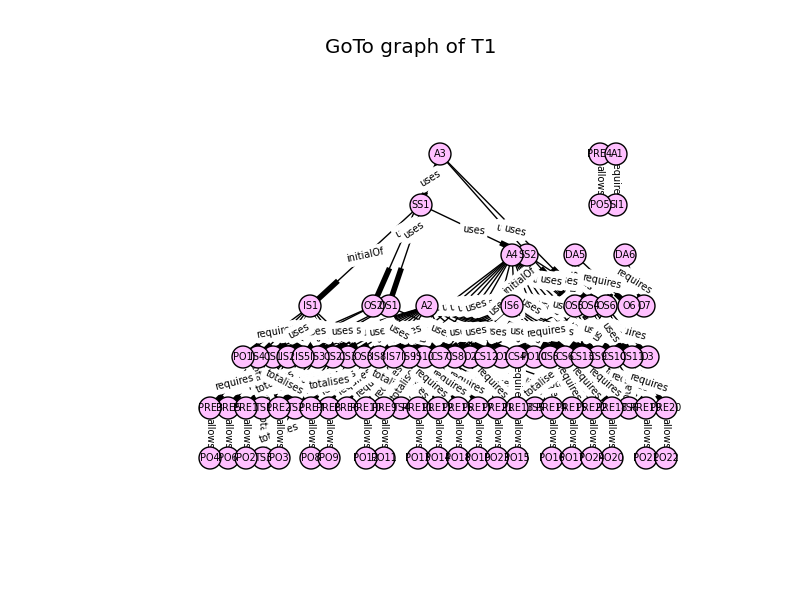
\includegraphics[trim=4cm 1cm 1cm 1cm, scale=0.5]{examples/steamboiler/25b.png}
\vspace{-0.2in}
\caption{The goto graph produced for the steamboiler specification. \label{fig:steamgotograph}}
\vspace{-0.2in}
\end{minipage}
\end{figure}

The dependecy and goto graphs are shown in figures \ref{fig:steamdepgrap} and \ref{fig:steamgotograph} respectively. Since there are a lot of \gls{zdra} instances and therefore a lot of nodes, both the dependecy graph and goto graph are cluttered. We will discuss this as a limitation in the next section.

From the goto graph the \gls{zmath} tool kit automatically generates a general proof skeleton, which uses the order from the goto graph to order the instances in how they should appear in any theorem prover. Part of the skeleton for the steamboiler specification is shown in figure \ref{fig:steamgpsa}.

\begin{figure}[H]
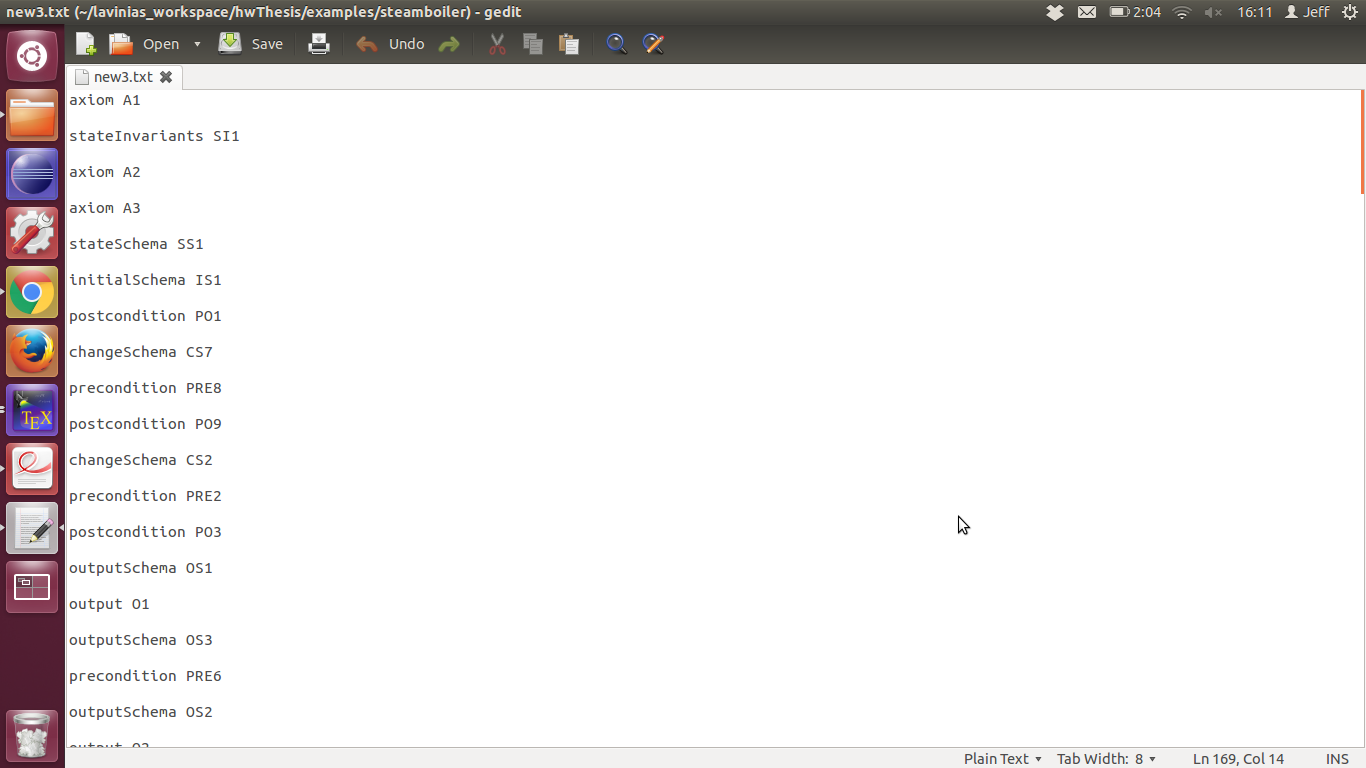
\includegraphics[scale=0.5]{Figures/Evaluation/steamboilergpsa.png}
\caption{\Gls{gps} for the steamboiler specification. \label{fig:steamgpsa}}
\end{figure}

We can now translate the \gls{gps} into Isabelle syntax using the \gls{zmath} toolkit.


\begin{figure}[H]
\centering
\begin{minipage}{0.43\textwidth}
\centering
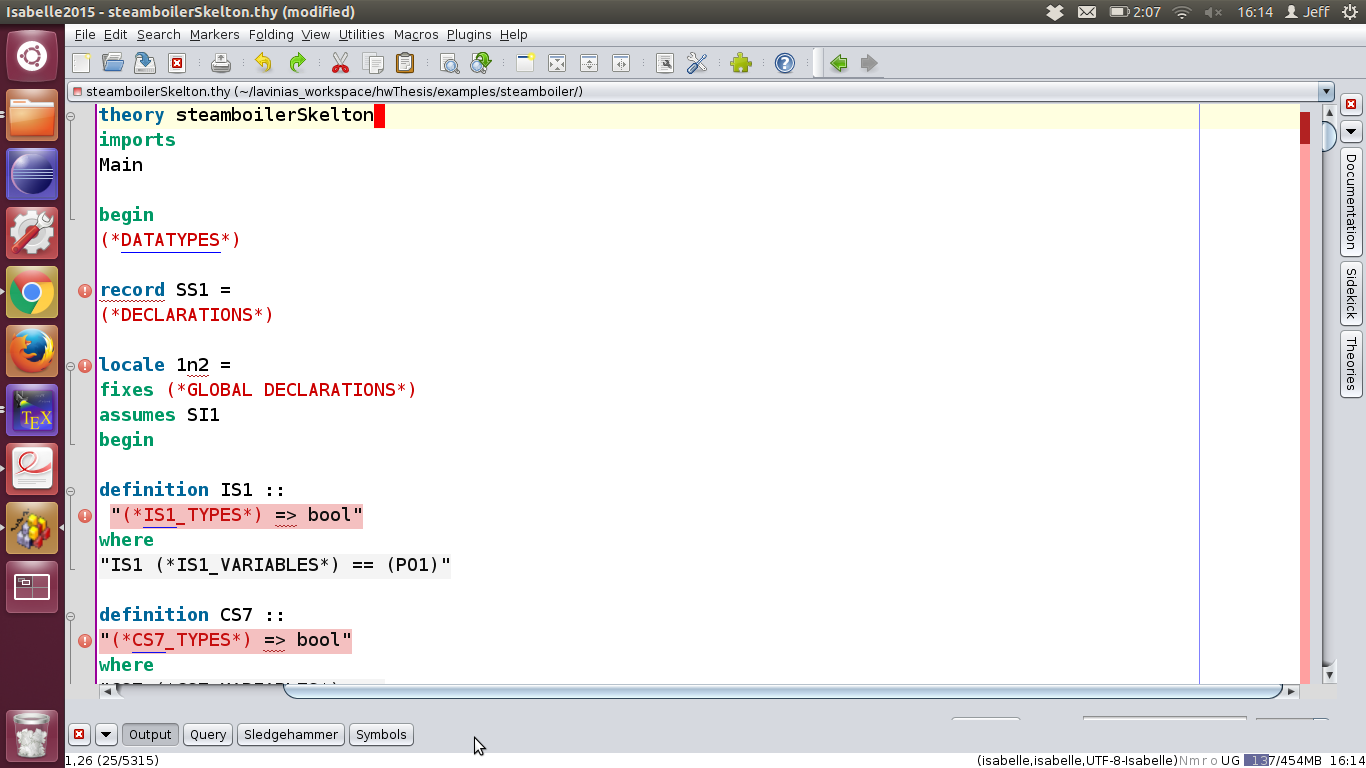
\includegraphics[ scale=0.5]{Figures/Evaluation/4image.png}
\end{minipage}\hfill
\begin{minipage}{0.53\textwidth}
%[clip,l,b,r,t]
\centering
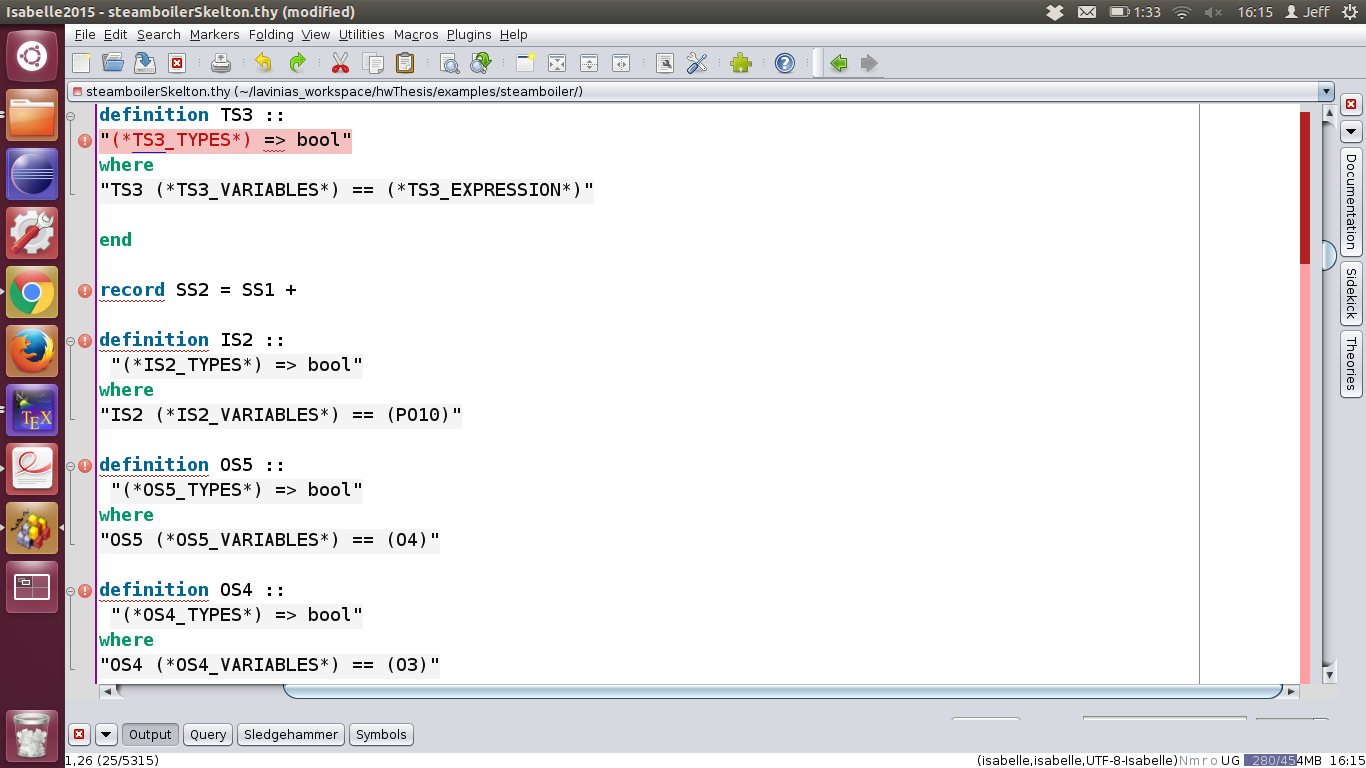
\includegraphics[scale=0.5]{Figures/Evaluation/4imageb.png}
\end{minipage}
\begin{minipage}{0.45\textwidth}
%[clip,l,b,r,t]
\centering
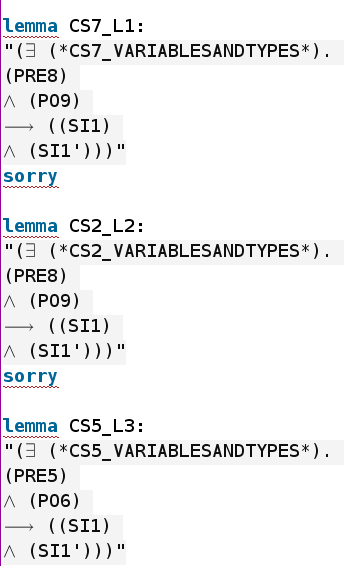
\includegraphics[scale=0.5]{Figures/Evaluation/4imagec.png}
\end{minipage}
\caption{Part of the isabelle skeleton for the steamboiler specification.\label{fig:steamisaskel}}
\end{figure}

Part of the isabelle skeleton for the steamboiler specification is shown in figure \ref{fig:steamisaskel}. Since the steamboiler example has 2 stateSchema's the \gls{zmath} toolset creates 2 isabelle 	\texttt{records} in the theory file. The top left image shows the beginning part of the isabelle skeleton, where the first stateSchema (or record) sets the state of the theory. Midway down the theory file the first record \texttt{ends} and a new one is added with the line \verb|record SS2 = SS1 +|. Towards the end the isabelle skeleton there are lemma's to check the consistency for all state changing schema's (\texttt{CS}) in the format decribed in chapter \ref{ch:skeletons} section \ref{subsec:pob1}. Using the \gls{zcga} annotated specification and the steamboiler isabelle skeleton, the \gls{zmath} tool support can now fill in the isabelle skeleton the declarations, expressions, schemaNames etc.


\begin{figure}[H]
\centering
\begin{minipage}{0.43\textwidth}
\centering
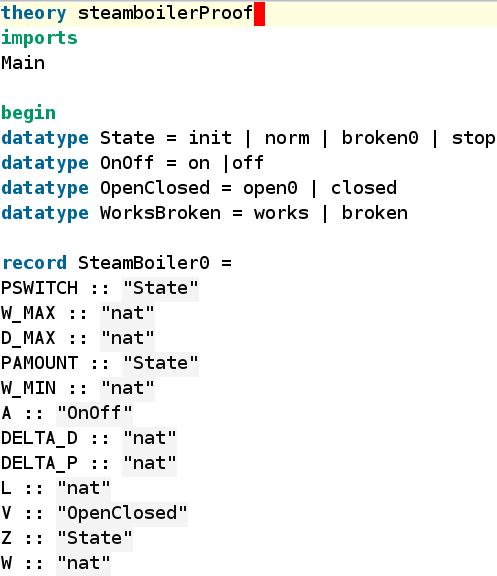
\includegraphics[ scale=0.4]{Figures/Evaluation/5imagea.png}
\end{minipage}\hfill
\begin{minipage}{0.53\textwidth}
%[clip,l,b,r,t]
\centering
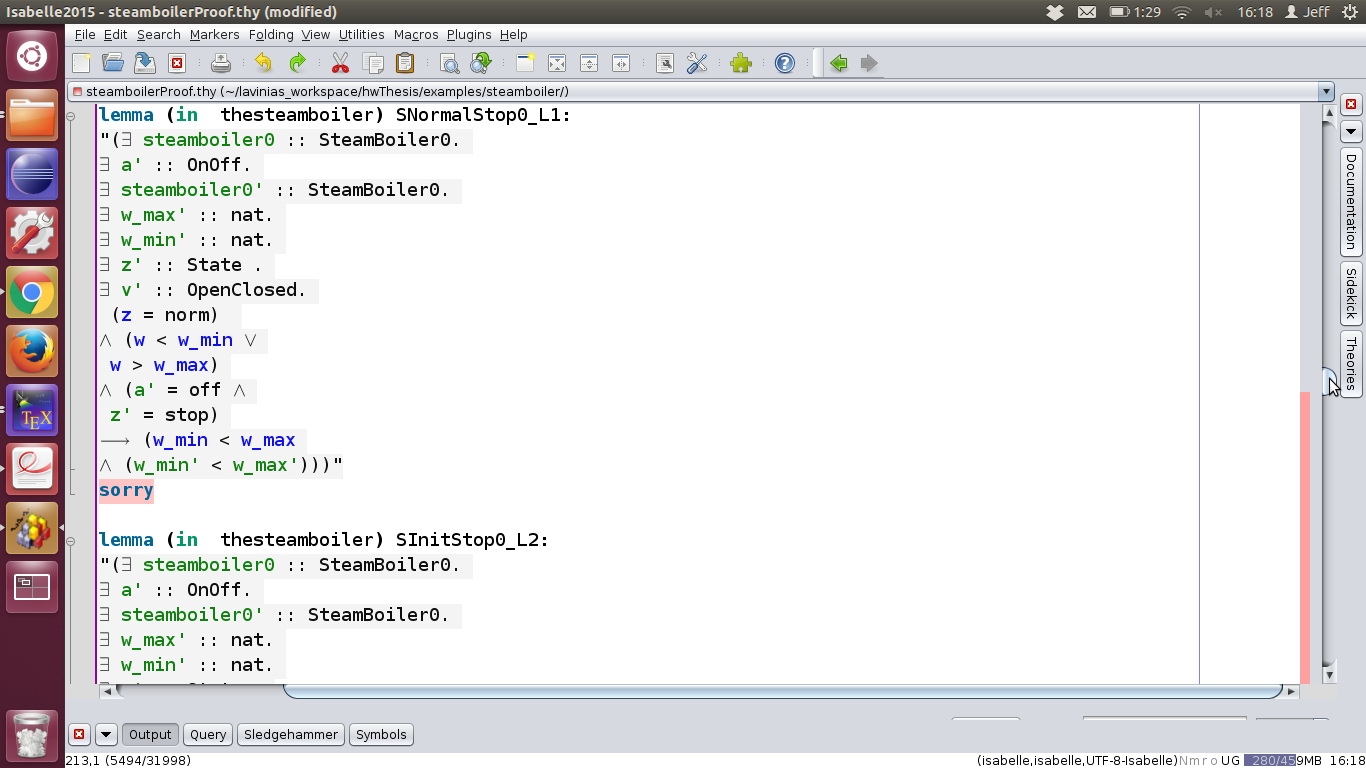
\includegraphics[scale=0.4]{Figures/Evaluation/5imagec.png}
\end{minipage}\hfill\hfill
%\begin{minipage}{0.7\textwidth}
%[clip,l,b,r,t]
%\centering
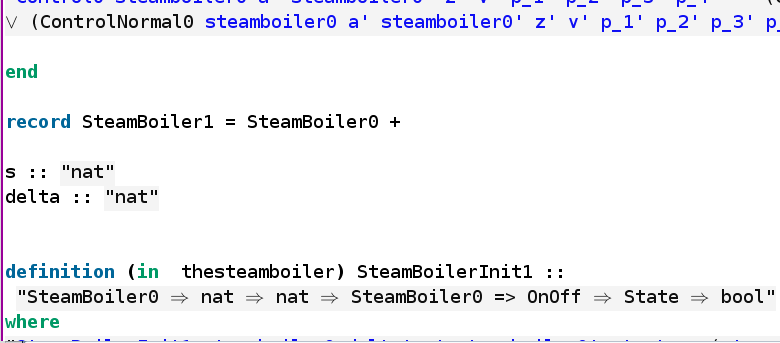
\includegraphics[scale=0.4]{Figures/Evaluation/5imageb.png}
%\end{minipage}
\caption{Part of the filled in isabelle skeleton for the steamboiler specification.\label{fig:filledinsteamskeleton}}
\end{figure}

In figure \ref{fig:filledinsteamskeleton} we show 3 parts of the filled in isabelle skeleton (\gls{half}). The first part shows the beginning of the \gls{half} which initiates the beginning of the proof. Since $SS1$ in this case was the root of the tree in the goto graph it sets \verb|SteamBoiler0| as the first record. Middway through the theory file we see another record, \verb|SteamBoiler1| which was $SS2$ in \gls{zdra}. This is shown in the bottom picture in figure \ref{fig:filledinsteamskeleton}. $SS2$ introduced 2 new state variables, $S$ and $delta$ which are added to the new record. Towards the end of the \gls{half}, \gls{zmath} has filled in the lemma's to prove which are sanity checks for the specification. It fills in the lemma's with the correct syntax so that the user only needs to delete the word `\emph{sorry}' prove the properties in order to get a proof of their specification. 

\begin{figure}[H]
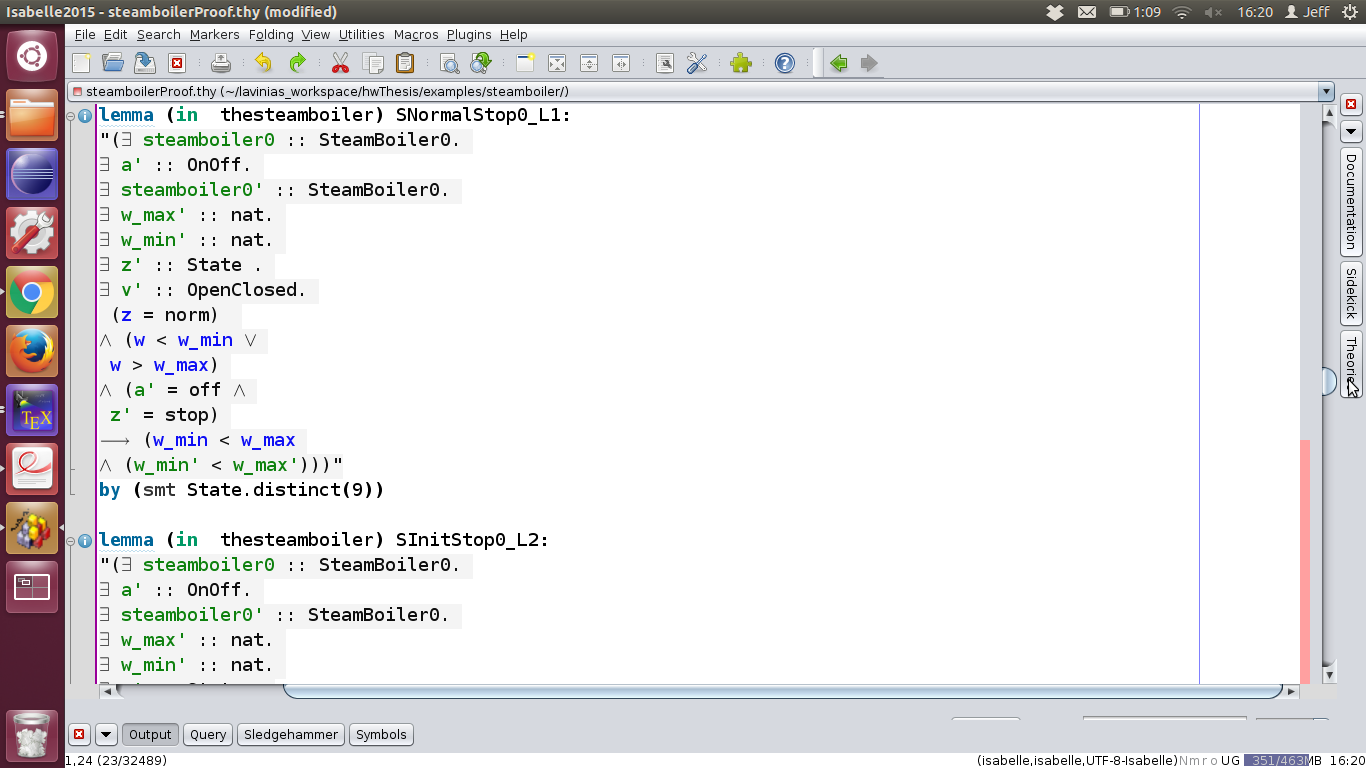
\includegraphics[scale=0.5]{Figures/Evaluation/6image.png}
\caption{Manually proven lemma for the steamboiler specification. \label{fig:steamboilerproof}}
\end{figure}

Using the lemma's which have been generated in figure \ref{fig:filledinsteamskeleton} we have proved all of these lemmas for the steamboiler specification, part of which is shown in figure \ref{fig:steamboilerproof}. By doing so, we have now proven that non of the state changing schemas conflict with the state invariants of the specification. To do this we have manually deleted the `\emph{sorry}' command, used the Isar tool `\emph{sledgehammer}' which has indicated that to prove this particular lemma (shown in figure \ref{fig:steamboilerproof}) it can be proven by \verb|smt State.distinct(9)|. Therefore it is true that the `\texttt{SNormalStop0}' schema does not conflict with the state Invariants. We did this step manually for all remaining lemmas, the full proof of the steamboiler specification can be found in \cite{mathlangexamples}.

\subsection{Case Study 2: A specification using both terms and sets.}

This case study based is on the \emph{ModuleReg} specification which uses both terms and sets. The specification has been translated into Isabelle using the \gls{zmath} framework. The entire \gls{zmath} works for the ModuleReg example is shown in chapter \ref{ch:fullexample}.

The \emph{ModuleReg} specification is our smallest example with 43 lines of \LaTeX{} code, 1 \emph{zed} environment and 3 \emph{schema}'s. There are 20 labels of \emph{schemaText}, 6 \emph{declarations}, 18 \emph{expressions}, 13 \emph{terms}, and 31 \emph{sets}. Since there are \emph{stateInvariants} for the \emph{modulereg} specification, \gls{zmath} was able to generate lemma's to prove for the 2 \emph{changeSchemas}. There is also 1 \emph{stateSchema}, 2 \emph{preconditions} and 2 \emph{postconditions}. There are 3 \emph{requires} relations, 2 \emph{allows} and 2 \emph{uses}.

Since the \emph{modulereg} specification is quite small but did have stateInvariants which \gls{zmath} could prove are satisfied throughout the specification, we decided it would be a could example to show the full workings of. This is shown in chapter \ref{ch:fullexample}.

\subsection{Case Study 3: A semi formal specification.}

In this case study we present the \emph{AutoPilot} specification. The specification is a semi formal specification and has been partially translated into Isabelle. The parts which have been translated are written formally and have been annotated accordingly. This gives an example of a specification which is written in natural language and is on it's way to being formalised.

We have taken the natural language specification for an autopilot system from \cite{Butler96} and started to formalise it.

\begin{figure}[H]
\centering
\begin{minipage}{0.45\textwidth}
\centering
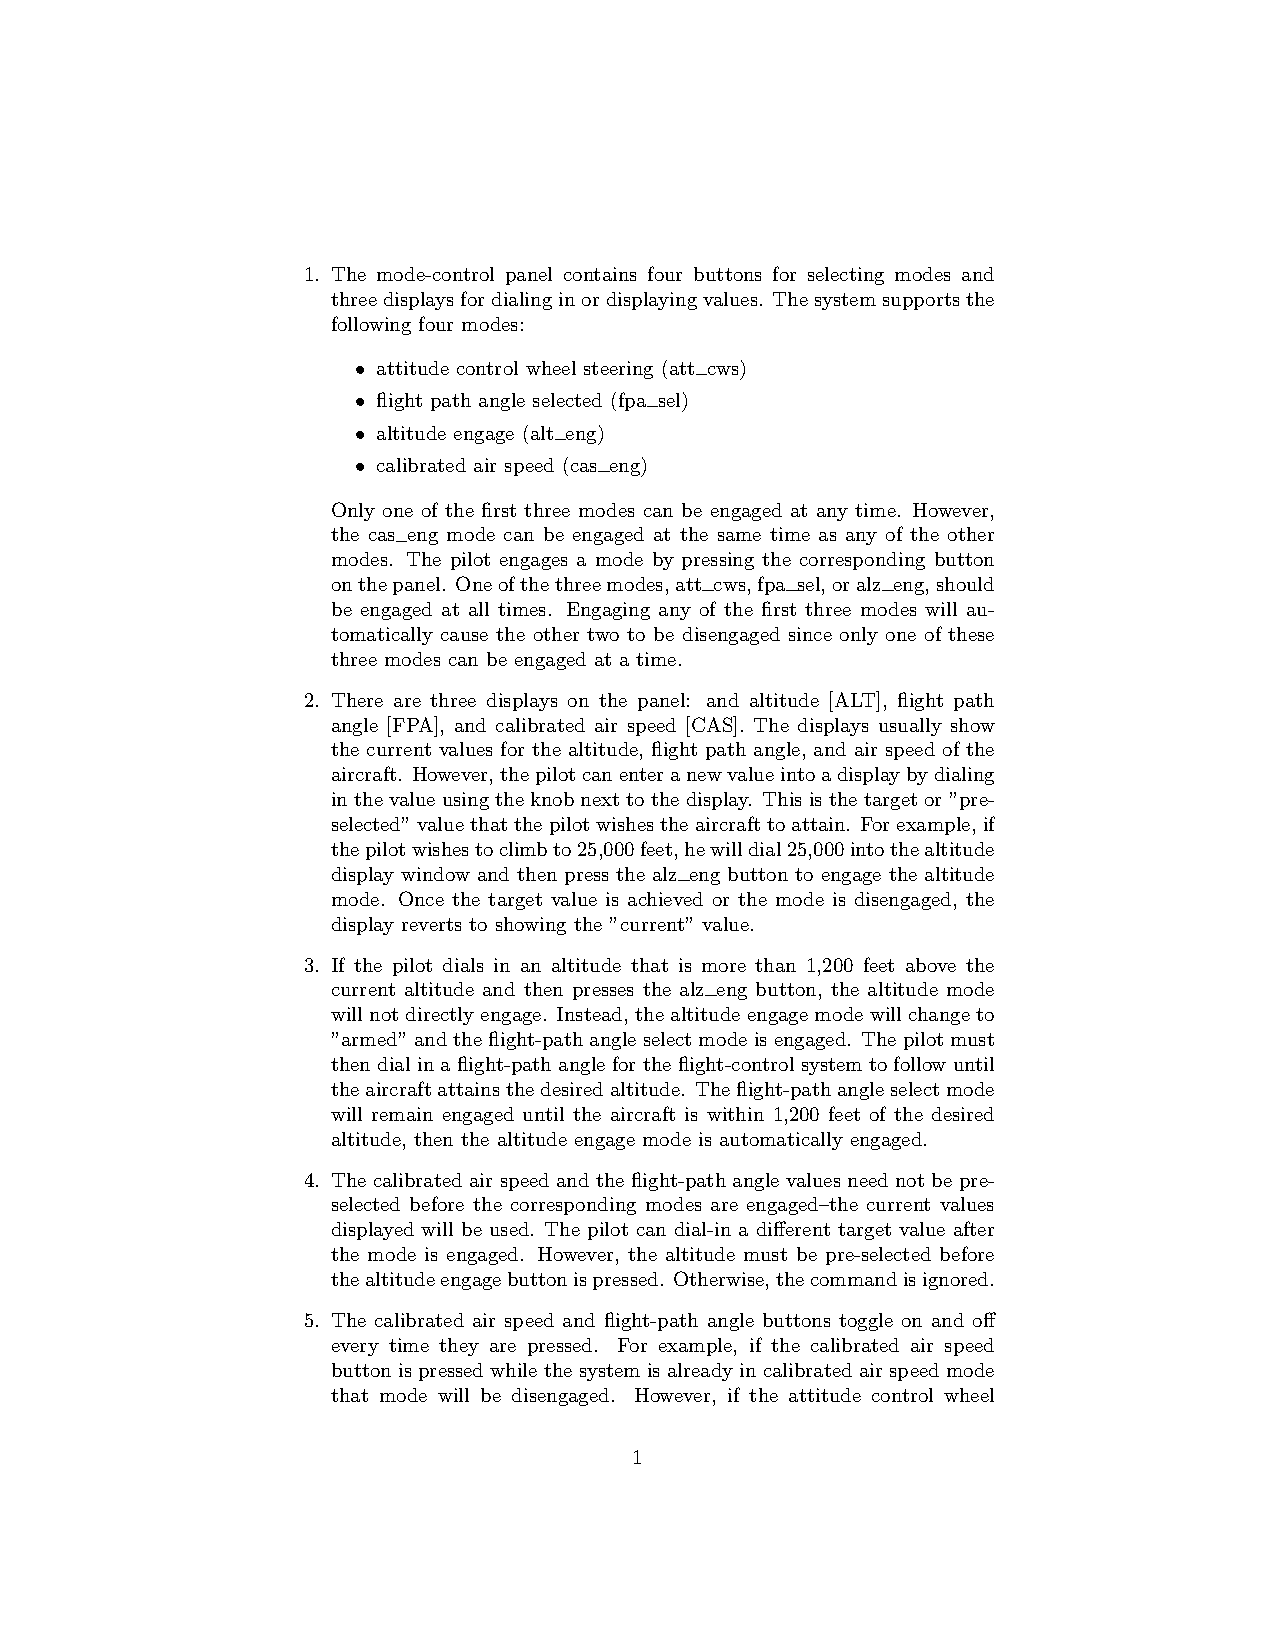
\includegraphics[clip, trim=5.5cm 11cm 4cm 4.5cm, scale=0.6]{examples/semiform/informal.pdf}
\vspace{-0.18in}
\caption{An example of the original Autopilot specification. \label{fig:originalautopilot}}
\vspace{-0.2in}
\end{minipage}\hfill
\begin{minipage}{0.45\textwidth}
\centering
%[clip,l,b,r,t]
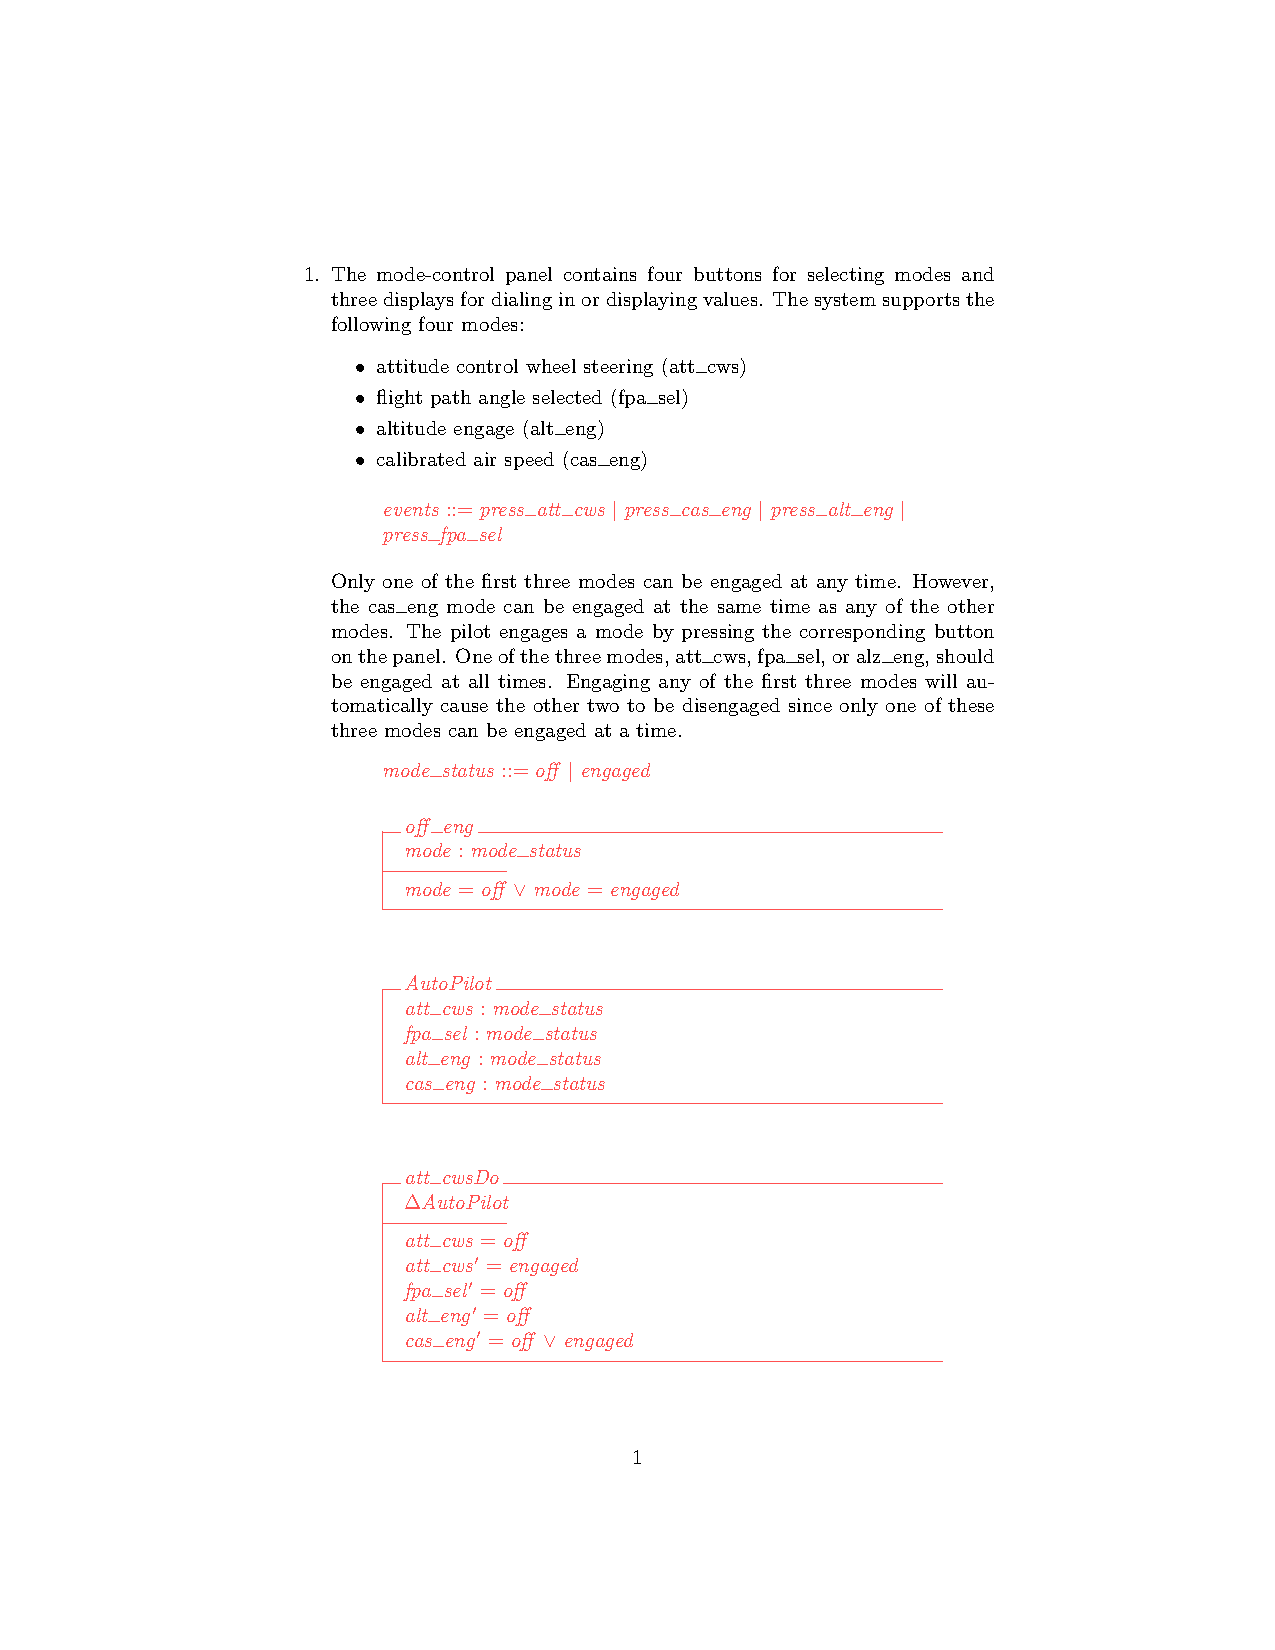
\includegraphics[clip, trim=5.5cm 11cm 4cm 4.5cm, scale=0.6]{examples/semiform/semiformal.pdf}
\vspace{-0.2in}
\caption{An example of the Autopilot specification partially formalised. \label{fig:semiformautopilot}}
\vspace{-0.2in}
\end{minipage}
\end{figure}

\subsubsection{ZMathLang steps for the autopilot case study.}

We give the informal specification in figure \ref{fig:originalautopilot} and one which we are beginning to formalised in figure \ref{fig:semiformautopilot}. We have highlighted in {\color{set}red} the parts which we have formalised in figure \ref{fig:semiformautopilot}. The formalised parts of the semi formal specification are taken from the text in the informal specification.

We then annotate the partial formal specification in \gls{zcga} annotations and \gls{zdra} annotations taken from chapters \ref{ch:zcga} and \ref{ch:zdra} respectively. Once annotated we can check the annotated document for \gls{zcga} and \gls{zdra} errors. 

\begin{figure}[H]
\centering
\begin{minipage}{0.45\textwidth}
\centering

\includegraphics[clip, trim=0cm 8cm 6cm 2cm, scale=0.6]{examples/semiform/1n2.pdf}
\vspace{-0.18in}
\caption{An example of the original Autopilot specification annotated in \gls{zcga} and \gls{zdra}. \label{fig:autopilot1n2}}
\vspace{-0.2in}
\end{minipage}\hfill
\begin{minipage}{0.45\textwidth}
\centering
%[clip,l,b,r,t]
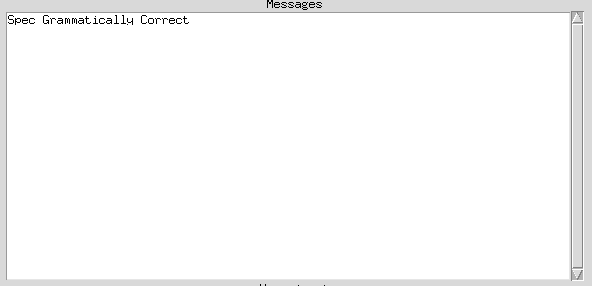
\includegraphics[clip, trim=0cm 8.5cm 9cm 0cm, scale=0.5]{examples/semiform/zcgacorrect.png}
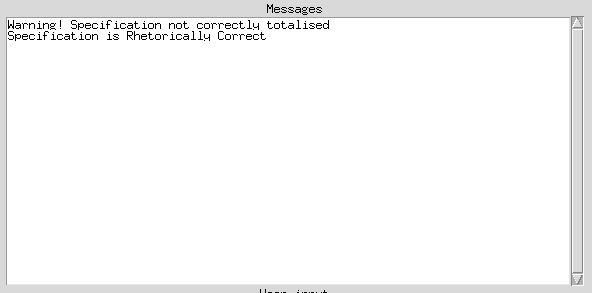
\includegraphics[clip, trim=0cm 8.5cm 9cm 0cm, scale=0.5]{examples/semiform/zdracorrect.png}
\vspace{-0.2in}
\caption{The outputting result when checking the autopilot specification with the \gls{zcga} and \gls{zdra} checkers. \label{fig:autopilotcorrect}}
\vspace{-0.2in}
\end{minipage}
\end{figure}

Even though the specification is not fully formalised we can still annotate it with \gls{zcga} and \gls{zdra} and check for the correctness of the parts which have been annotated (shown in figures \ref{fig:autopilot1n2} and \ref{fig:autopilotcorrect}). When checking with \gls{zdra} we have a warning message telling the user that the specification is not correctlty totalised. That is there is a precondition outstand with not postcondition counter part. This does not matter for now as we can still carry on with the tranlation.

When checking the specification for \gls{zdra}, \gls{zmath} has also produced a dependecy graph and goto graphs (shown in figures \ref{fig:autodepgraph} and \ref{fig:autogotograph}):

\begin{figure}[H]
\centering
\begin{minipage}{0.45\textwidth}
\centering
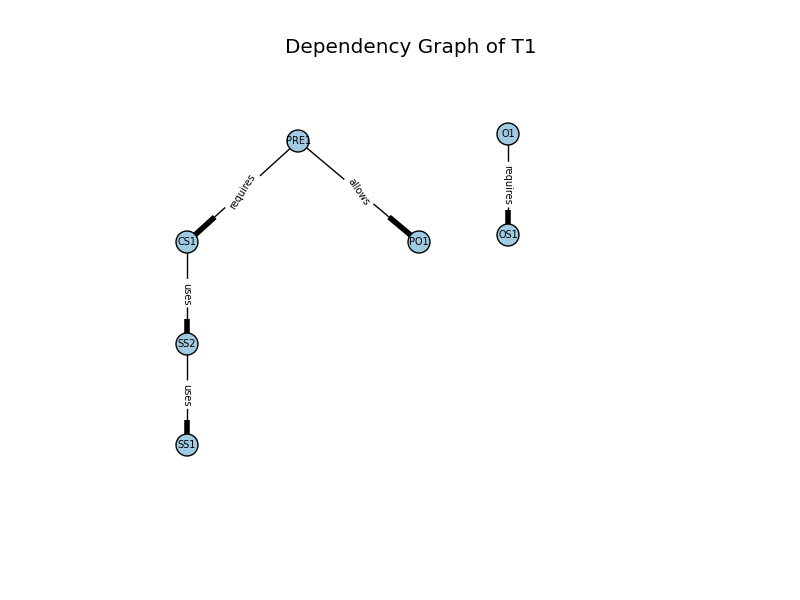
\includegraphics[scale=0.5]{examples/semiform/25a.png}
\vspace{-0.18in}
\caption{The dependecy graph produced for the autopilot specification. \label{fig:autodepgraph}}
\vspace{-0.2in}
\end{minipage}\hfill
\begin{minipage}{0.43\textwidth}
\centering
%[clip,l,b,r,t]
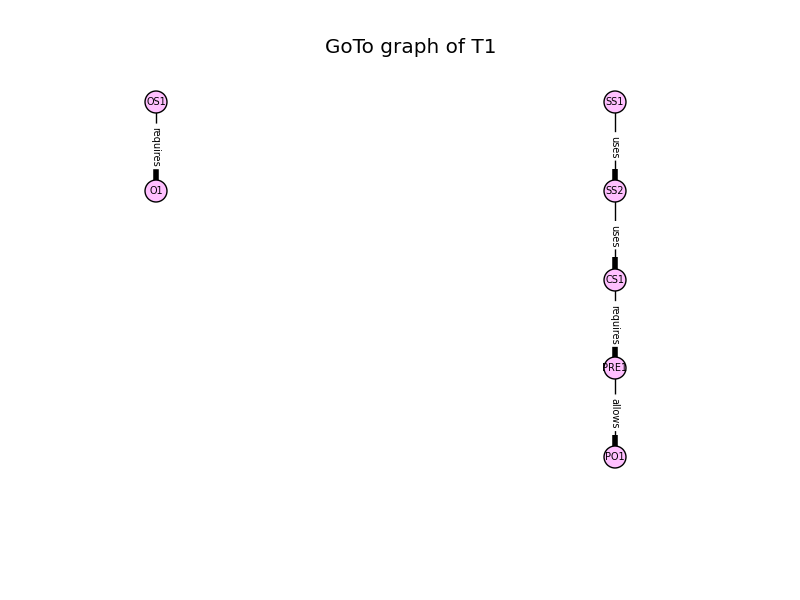
\includegraphics[scale=0.5]{examples/semiform/25b.png}
\vspace{-0.2in}
\caption{The goto graph produced for the autopilot specification. \label{fig:autogotograph}}
\vspace{-0.2in}
\end{minipage}
\end{figure}

With the dependency graph (figure \ref{fig:autodepgraph}) we can say that $SS2$ uses $SS1$, $CS1$ uses $SS2$, $PRE1$ requires $CS1$ and allows $PO1$. Which makes up the main tree dependencies. $OS1$ and $O1$ are seperate as they do not have any relations which any parts of the main tree, the only dependency they have is on eachother where $O1$ requires $OS1$.

We can say that the dependecy graph \emph{describes} the relation between instances and the goto graph (figure \ref{fig:autogotograph}) \emph{orders} the instances in a way as to parse through a theorem prover.

We can now generate a general proof skeleton for the Autopilot specification even though it is not fully formalised (shown in figure \ref{fig:autopilotgps}). We can clearly see that the arrow has changed direction for the $OS1$ and $O1$ relationship from the dependency graph. Again since these two instances are not dependency on any part of the main tree they are seperate. However in the dependency graph described the relation that $O1\ requires\ OS1$ ($O1$ root and $OS1$ child) the goto graph flips this relationship as in a theorem prover we woud need $OS1$ to appear before $O1$ since $O1$ requires $OS1$ to exist. We can also say that $SS2$ uses $SS1$ therefore $SS2$ needs $SS1$ to exist for itself to exist. Then $CS1$ uses $SS2$ therefore $CS1$ needs $SS2$ to exist for itself to exit. We can say that $PRE1$ requires $CS1$ and allows $PO1$. Thefore $PO1$ needs $PRE1$ to exist before it is allowed to exist itself.

\begin{figure}[H]
\centering
\begin{center}
\begin{verbatim}
stateSchema SS1 
outputSchema OS1 
output O1 
stateSchema SS2 
changeSchema CS1 
precondition PRE1 
postcondition PO1 
\end{verbatim}
\end{center}
\caption{\Gls{gps} for the Autopilot specification. \label{fig:autopilotgps}}
\end{figure}

Since the Autopilot specification has passed the \gls{zcga} and \gls{zdra} checks we can then generate a \gls{gps} for the specification using the goto graph produced in the previous stage. The way this is done is described in section \ref{sec:zdra2gen}. Note that even though there is a $changeSchema$ instance, there are no $stateInvariants$ in the specification (as yet). Therefore \gls{zmath} does not generate any lemma's to prove in this case since \gls{zmath} only checks for consistancy accross the specification and thus need state invariants to be present.

\begin{figure}[H]
\centering
\begin{minipage}{0.45\textwidth}
\centering
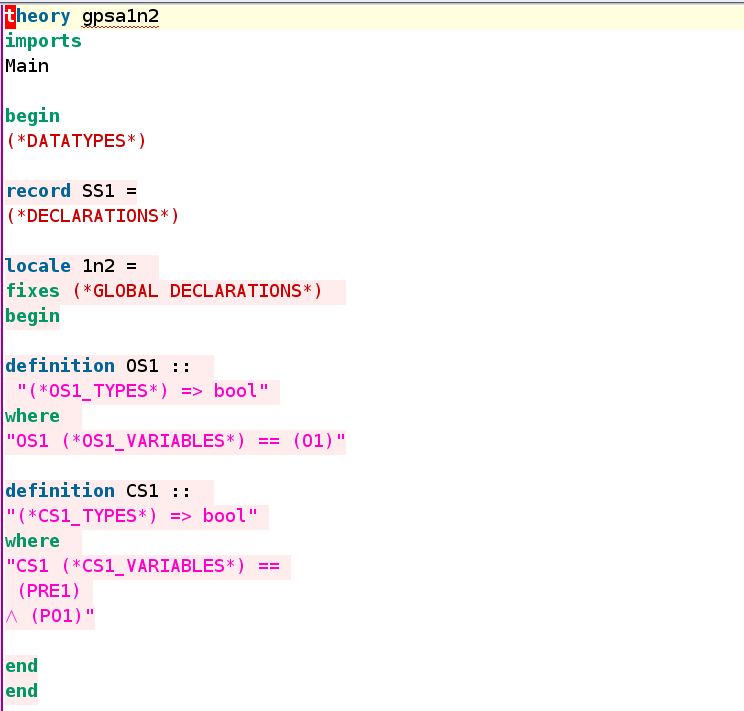
\includegraphics[clip, trim=0cm 0cm 15cm 0cm, scale=0.5]{examples/semiform/4image.png}
\vspace{-0.18in}
\caption{The Isabelle skeleton produced for the autopilot specification. \label{fig:autoisskel}}
\vspace{-0.2in}
\end{minipage}\hfill
\begin{minipage}{0.43\textwidth}
\centering
%[clip,l,b,r,t]
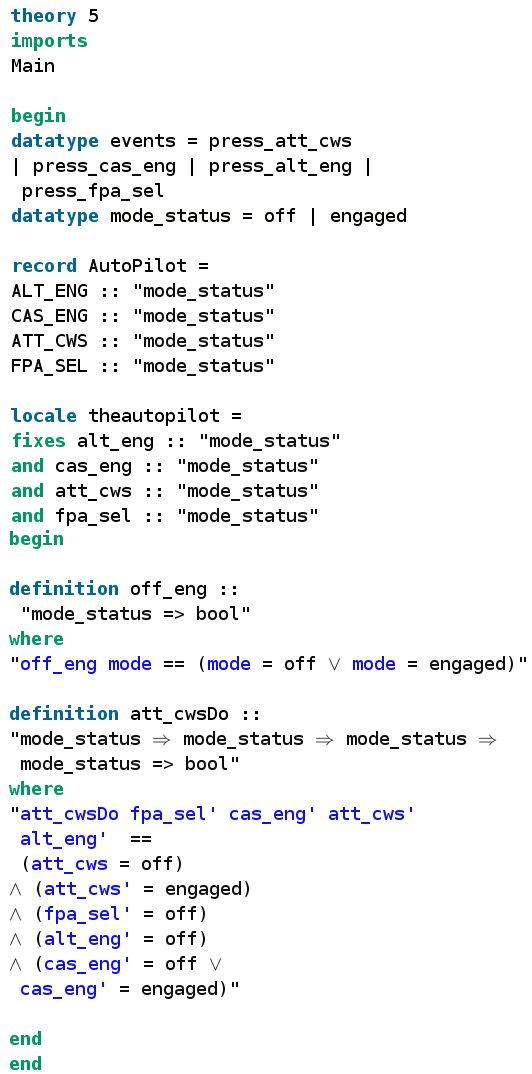
\includegraphics[clip, trim=0cm 0cm 4cm 0cm, scale=0.35]{examples/semiform/5imageal.png}
\vspace{-0.2in}
\caption{The autopilot specification in Isabelle syntax. \label{fig:autoisa}}
\vspace{-0.2in}
\end{minipage}
\end{figure}

\Gls{zmath} can automatically translate the \gls{gps} into Isabelle syntax (figure \ref{fig:autoisskel}), this is now an Isabelle skeleton. The Isabelle skeleton has not yet taken the \gls{zcga} information as one can get to this step with just the \gls{zdra} annotated document. Once the Isabelle is filled in (figure \ref{fig:autoisa}) we have the annotated specification in Isabelle form. This can now give the user an idea of how to input their specifiation into Isabelle syntax, without them having prior knowledge of Isabelle. It is important to note that this is as far as the \gls{zmath} translation goes. Since there are no state Invariants with this case study no lemma's to check for consistancy have been generated. The user can add the state Invariants in their raw \LaTeX{} specification, or fully formalise their specification. Another way to fully prove their specification is to add other properties to the Isabelle document.

\section{Analysing examples}

In this section we analyse the examples we have successfully translated into Isabelle and proved the sanity of the specification. 


We remind the reader of figure \ref{fig:timeline} in chapter \ref{ch:design}. \Gls{zmath} is able assit the user with the translation of specification up to the point where sanity properties are produced but not proven. In our largest case study (section \ref{subsec:casestudy1}) the user did not have to look through all the state changing schema's and write the sanity checks for all of them. The properties were already generated for each changeSchema however, the user did have to go through each property and prove it. In total, there were 21 changeSchema's and 1 set of stateInvariants, therefore there was 21 properties which the user had to prove manually.

\subsection{SteamBoiler}

In our largest example there were 21 changeSchema's and 1 set of stateInvariants, therefore there was 21 properties which the user had to prove manually.

To prove the sanity of the steamboiler specification, we went through the consistency lemmas (automatically generated) one by one and manually prove them. We started of with unproven lemma's with the command `\emph{sorry}' at the end such as the lemma shown in figure \ref{fig:steamboilerL1lemma}.

\begin{figure}[H]
\centering
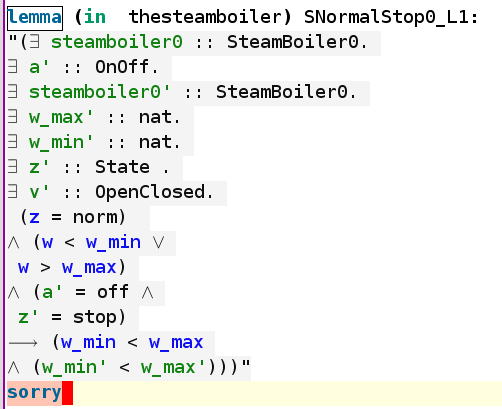
\includegraphics[scale=0.5]{Figures/Evaluation/sorryoutputlemma.png}
\caption{The `\texttt{SNormalStop0}' lemma taken from the steamboiler \gls{half}. \label{fig:steamboilerL1lemma}}
\end{figure}

We then delete the `\emph{sorry}' command and if sledgehammer is set up to be automatic, the user can sometimes leave their cursor at the end of the lemma and `\emph{auto sledgehammer}' finds a proof which is displayed in the output terminal. In our case, this has happened for the `\texttt{SNormalStop0}' lemma which is displayed in figure \ref{fig:autosolvelemma}.

\begin{figure}[H]
\centering
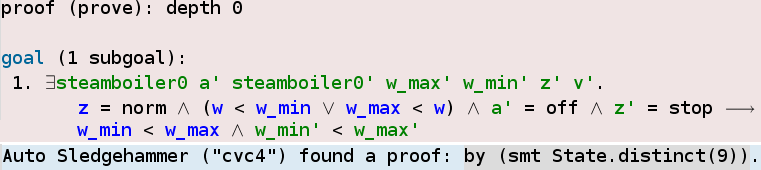
\includegraphics[scale=0.5]{Figures/Evaluation/steamboilerlemmaproof.png}
\caption{Auto sledgehammer finding a proof for one of the lemma's in the steamboiler specification using the \gls{smt} solver `\emph{cvc4}'. \label{fig:autosolvelemma}}
\end{figure}

In this particular lemma we are proving the property that the \verb|SNormal_Stop)| schema does not conflict with the state invariants of the specification either before or after the state has been changed. Some other lemma's in the steamboiler example (such as the \verb|SInitNormal1_L9| lemma) could be proven by the isabelle command `\texttt{blast}' as shown in figure \ref{fig:blastprovenlemma}. 

\begin{figure}[H]
\centering
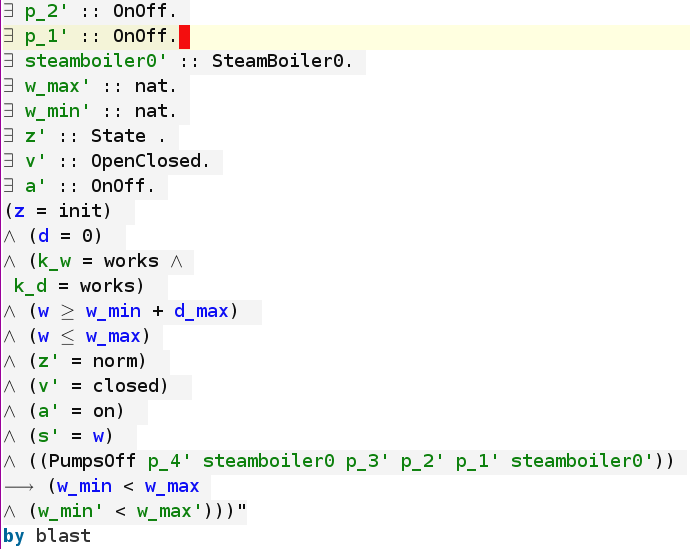
\includegraphics[scale=0.6]{Figures/Evaluation/steamboilerblastlemma.png}
\caption{An example of a lemma in the steamboiler specification being proved by blast. \label{fig:blastprovenlemma}}
\end{figure}

Proving by `\emph{blast}' is obviously less complex then the proof needed for lemma \verb|SNormalStop0_L1| in figure \ref{fig:steamboilerL1lemma}, however if we look back to figure \ref{fig:timeline} in chapter \ref{ch:design} we can see that `\emph{blast}' covers less properties then `\emph{sledgehammer}'. Therefore for the lemma's in the steamboiler specification we have proved 2 lemma's by blast and 19 using sledgehammer. 

It is important to note that a single lemma can be proven in a variety of ways, so even thoguh we have chosen to prove our specification in certain ways other users may choose to use other tools to prove their theorems and lemmas. Even though we have proved 19 lemmas by sledgehammer in the steamboiler specification, we might have been able to prove all the lemmas by sledgehammer but chosen to prove 2 by blast to show variety.

\subsection{ModuleReg}

The modulereg is one of our smallest examples, however with 1 set of stateinvariants and 2 changeSchemas, \gls{zmath} automatcally produces 2 lemma's to check the sanity of the specification. An example of one of these lemmas is shown in figure \ref{fig:modulereglemma1}. This is one of the lemma's automatically generated and thus we have the `\emph{sorry}' command at the end to show that it needs manual input from the user to complete the proof.

\begin{figure}[H]
\centering
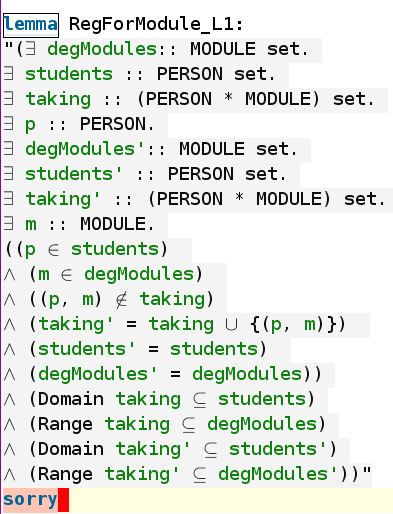
\includegraphics[scale=0.5]{Figures/Evaluation/lemmaformodulereg.png}
\caption{An example of one of the lemma's to check for consistency in the modulereg specification. \label{fig:modulereglemma1}}
\end{figure}

To prove this lemma we remove the `\emph{sorry}' command or put our curser at the end of the lemma ready to input our methods to start the proof. In this case `\emph{Auto sledgehammer}' again found a proof using the `\texttt{cvc4}' \gls{smt} solver (shown in figure \ref{fig:autosolvermodulereg}). With this lemma we are aiming to prove the sanity of the specification where the changeSchema \verb|RegForModule| does not conflict with the stateInvariants either before or after the state has been changed.

\begin{figure}[H]
\centering
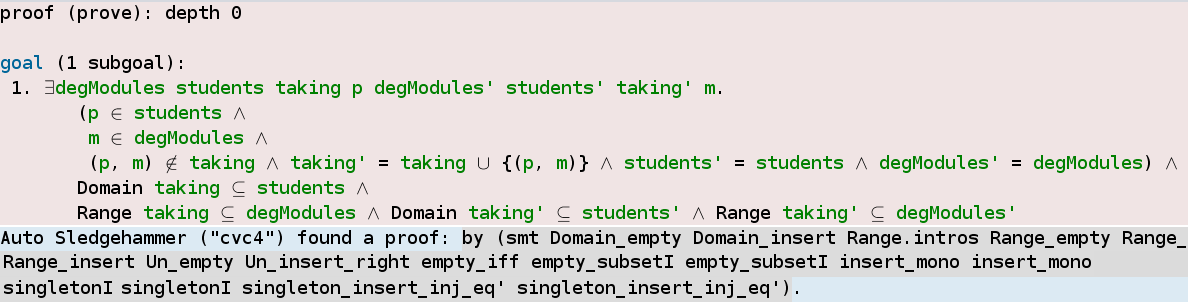
\includegraphics[scale=0.35]{Figures/Evaluation/moduleregproof.png}
\caption{Output shown when proving the lemma `\texttt{RegForModule} shown in figure \ref{fig:modulereglemma1} . \label{fig:autosolvermodulereg}}
\end{figure}

By clicking on the auto solving method shown in figure \ref{fig:autosolvermodulereg} we can now complete the proof for the \verb|RegForModule_L1| lemma. This is shown 

\begin{figure}[H]
\centering
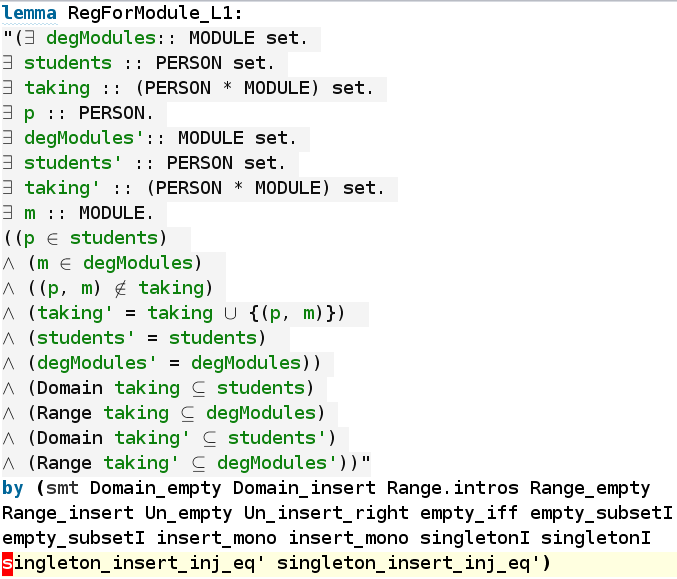
\includegraphics[scale=0.5]{Figures/Evaluation/provenmodulelemma.png}
\caption{The `\texttt{RegForModule}' lemma proved using Auto sledgehammer methods. \label{fig:solvedmodulelemma}}
\end{figure}

The second lemma in the moduleReg specification we managed to prove using `\emph{blast}' thus having a complete proof for the complexity of the modulereg specification.

We can see that the complexity of the proof used for the \verb|RegForModule_L1| lemma in the modulereg specification is larger than the complexity of the proof for the \verb|SNormalStop0_L1| in the steamboiler specification. Although we used `\emph{Auto sledgehammer}' to assist proving the lemma's there are 16 methods used in proving the \verb|RegForModule_L1| lemma (\verb|Domain_empty|, \verb|Range_empty| etc.) compared with 1 method used in proving the \verb|SNormalStop0_L1| lemma (\verb|State.distinct(9)|). Again we can say that there might of been an alternate way to prove these particular lemma's however we have chosen to prove them in this way to show variation. Since there are more state changing schema's in the steamboiler specification there are also more lemma's to prove with the steamboiler then there is in the modulereg specification to obtain a fully proven specification which checks the complexity of the system.

\subsection{Vending Machine}

The vending machine example has 3 state changing schemas (shown in table \ref{tab:speczdracount}) however since it does not have any labeled stateInvariants, \gls{zmath} can not automatically produce any properties to prove the consistency of the specification. If we refer back to figure \ref{fig:timeline} in chapter \ref{ch:design} it shows that the \gls{zmath} toolkit goes slightly past the point of `\emph{specification in isabelle with no proof}' however the automation of \gls{zmath} can only go past that point \textbf{if} there are changeschema's and stateInvariants labelled. Otherwise the \gls{zmath} toolkit can only translate the specification into isabelle syntax with no lemma's or properties to prove. Thus it is up to the user to carry on manually inputting their properties to obtain a fully proven specification.

\subsection{Other examples}

Each specification has a different amount of lemma's which the user needs to prove depending on how many `stateInvariants' and `changeSchema's' there are. If the specification does not have any stateInvariants then \gls{zmath} will not produce any lemmas to prove for the sanity of the specification.

\begin{table}
\begin{tabular}{|l | l | l |}
\hline
\textbf{Specification} & \textbf{Amount of} & \textbf{Total amount} \\
& \textbf{generated lemmas} & \textbf{of tactics} \\
\hline
Steamboiler & 20 & 41 \\
ProjectAlloc & 5 & 18 \\
VideoShop & 3 & 3 \\
TelephoneDirectory & 4 & 8 \\
ClubState & 4 & 4 \\
ZCGa & 6 & 6 \\
GenDB & 4 & 13 \\
Timetable & 4 & 4 \\
BirthdayBook & 1 & 1\\
AutoPilot & 0 & 0 \\
ClubState2 & 3 & 4 \\
Vending Machine & 0 & 0 \\
ModuleReg & 2 & 18 \\
\hline
\end{tabular}
\caption{A table to show the amount of automatically generated lemmas and total amount of tactics used for each specification. \label{tab:lemmatact}}
\end{table}

We show the amount of lemmas and total amount of tactics needed to prove the sanity of each specification in table \ref{tab:lemmatact}. Some lemma's need only one tactic to be proved whilst other need a few. There are various different ways to prove these lemmas and it all comes down to the personal preference of the user. We have mainly used Isabelles `\emph{sledgehammer}' tool to assist us with our proving.

\subsubsection{SteamBoiler}

The steamboiler has in total 20 lemmas to check the specifications sanity as it has 20 changing state schemas. The specification has 1 set of stateInvariants and we used 41 tactics to prove our lemmas.

The steamboiler state invariants is shown in the expression part of the stateSchema. The state invariants for this specification is that the minimum water level (\verb|w_min|) must be smaller than the maximum water level (\verb|w_max|). Therefore, the state invariants are writter after `\texttt{assumes}' in the specification (\verb|w_min < w_max|). 

When \gls{zmath} produces the proof obigations to check the sanity of the specification it must also check that the changeSchema does not conflict with the prime state invariants. Thus, the proof obligations to check for all changing state schema will check that the preconditions and postconditions of each changeSchema still imply that (\verb|w_min < w_max|) \textbf{and} (\verb|w_min' < w_max'|).

For example to prove our first lemma \verb|SNormalStop0_L1|, we wish to make sure that the \verb|SNormalStop0| changeSchema does not conflict with the stateInvariants and the stateInvariants prime.

\noindent \begin{tabular}{|l | l|}
\hline
\verb|lemma (in  thesteamboiler)| & {\color{red}begin} \\
\verb|SNormalStop0_L1:|& {\color{red}Name of lemma} \\
\verb|"(\<exists> steamboiler0 :: | & \\
\verb|SteamBoiler0.|&  {\color{red}list of all} \\
\verb|\<exists> a' :: OnOff.|&  {\color{red}variables and} \\
\verb|\<exists> steamboiler0' :: | & {\color{red}types} \\
\verb|SteamBoiler0.|&  \\
\verb|\<exists> w_max' :: nat.|&  \\
\verb|\<exists> w_min' :: nat.|&  \\
\verb|\<exists> z' :: State.|&  \\
\verb|\<exists> v' :: OpenClosed.|&  \\
\verb|(z = norm)|&  {\color{red}preconditions \textbf{and}}\\
\verb|\<and> (w < w_min ∨|& {\color{red}postconditions of} \\
\verb|w > w_max)|& {\color{red}SNornalStop0 schema} \\
\verb|\<and> (a' = off \<and>|&  \\
\verb|z' = stop)|&  \\
\verb|\<longrightarrow> (w_min < w_max|& {\color{red}\textbf{implies} stateInvariants} \\
\verb|\<and> (w_min' < w_max')))"|& {\color{red}\textbf{and} stateInvariants prime} \\
\verb|by (smt State.distinct(9))|&  \\
\hline
\end{tabular}

Since there are 2 records in our steamboiler specification we have to manually write the line \verb|(in thesteamboiler)| which lets isabelle know that the changeSchema uses variables from the first record. The \verb|SNormalStop0_L1| lemma is proved using 2 tactics \verb|smt| and \verb|State.distinct(9)|. We remind the reader that although we have used these 2 tactics to prove our lemma there may be other ways in which to do so. 

Our most complex proof is for the \verb|SNormalContinue1_L11| lemma in which we use 3 tactics to prove the property that the \verb|SNormalContinue1| changeSchema does not conflict with the state Invariants. The tactics we use here are \verb|smt|, \verb|OnOff.distinct(1)| and \verb|pswitch.simps(1)|.

\subsubsection{ProjectAlloc}

The projectAlloc specification has 5 changeSchema's and 1 set of stateInvariants therefore it has 5 lemmas which \gls{zmath} has automatically generated to check for the consistancy. To prove these lemmas we have in total used 18 tactics.

The lemmas to check that the changeSchema's did not conflict with thestateInvariants with were as follows:

\begin{verbatim}
\<exists> variables and types.
Preconditions
\<and>
PostConditions
\<longrightarrow>
(((dom studInterests) \<inter> (dom lecInterests) = {})
\<and> (dom allocation \<subseteq> dom studInterests)
\<and> (ran allocation \<subseteq> dom lecInterests)
\<and> (dom maxPlaces = dom lecInterests)
\<and>  (\<forall> lec \<in> dom maxPlaces.
(card ({l. the (allocation l) = lec})) \<leq> the (maxPlaces lec))
\<and>  ((dom studInterests') \<inter> (dom lecInterests') = {})
\<and> (dom allocation' \<subseteq> dom studInterests')
\<and> (ran allocation' \<subseteq> dom lecInterests')
\<and> (dom maxPlaces' = dom lecInterests')
\<and>  (\<forall> lec \<in> dom maxPlaces'.
(card ({l. the (allocation' l) = lec})) \<leq> the (maxPlaces' lec))))"
\end{verbatim}

Our most complex lemma to prove is the \verb|AddLecturer_L5| lemma which we used 9 tactics. The most simple lemma to prove was \verb|AddStudent_L3| and \verb|DeAllocate_L2| where we just used 1 tactic (\verb|fastforce| and \verb|auto| respectively).

%\begin{tabular}{|l l |}
%\hline
%\verb|lemma AddLecturer_L5:| & \\
%\verb|"(\<exists> projectalloc :: ProjectAlloc.| & \\
%\verb|\<exists> projectalloc' :: ProjectAlloc.| & \\
%\verb|\<exists> studInterests' :: (PERSON \<rightharpoonup> ((nat * TOPIC) set)).| & \\
%\verb|\<exists> lecInterests' :: (PERSON \<rightharpoonup> ((nat * TOPIC) set)).| & \\
%\verb|\<exists> allocation' :: (PERSON \<rightharpoonup> PERSON).| & \\
%\verb|\<exists> maxPlaces' :: (PERSON \<rightharpoonup> nat).| & \\
%\verb|\<exists> l :: PERSON.| & \\
%\verb|\<exists> maxAlloc :: nat.| & \\
%\verb|\<exists> ts :: ((nat * TOPIC) set).| & \\
%\verb|(l \<notin> ((dom studInterests) \<union> (dom lecInterests)))| & \\
%\verb|\<and> (lecInterests' = lecInterests(l \<mapsto> ts))| & \\
%\verb|\<and> (maxPlaces' = maxPlaces(l \<mapsto> maxAlloc))| & \\
%\verb|\<and> (studInterests' = studInterests)| & \\
%\verb|\<and> (allocation' = allocation)| & \\
%\verb|\<longrightarrow>(((dom studInterests) \<inter> (dom lecInterests) = {})| & \\
%\verb|\<and>(dom allocation \<subseteq> dom studInterests)| & \\
%\verb|\<and>(ran allocation \<subseteq> dom lecInterests)| & \\
%\verb|\<and>(dom maxPlaces = dom lecInterests)| & \\
%\verb|\<and> (\<forall> lec \<in> dom maxPlaces. (card ({l. the (allocation l) = lec})) \<leq> the (maxPlaces lec))| & \\
%\verb|∧ ((dom studInterests') \<inter> (dom lecInterests') = {})| & \\
%\verb|∧(dom allocation' \<subseteq> dom studInterests')| & \\
%\verb|∧(ran allocation' \<subseteq> dom lecInterests')| & \\
%\verb|∧(dom maxPlaces' = dom lecInterests')| & \\
%\verb|∧ (\<forall> lec \<in> dom maxPlaces'. (card ({l. the (allocation' l) = lec})) \<leq> the (maxPlaces' lec))))"| & \\
%\verb|by (metis (full_types) dom_empty dom_empty dom_empty| & \\ \verb|dom_eq_singleton_conv dom_restrict inf.idem insert_not_empty)| & \\
%\end{tabular}

\subsubsection{VideoShop}

\subsubsection{TelephoneDirectory}

\subsubsection{ClubState}

\subsubsection{ZCGa}

\subsubsection{GenDB}

\subsubsection{Timetable}

\subsubsection{BirthdayBook}

\subsubsection{ClubState2}

\subsubsection{ModuleReg}

\section{Reflection and Discussion}

% Any assumptions  made

%reflect on the amount and complexity of manual proof still needed, and in particular whether this should
%be within grasp of a software/system designer, who is not necessarily an expert in Isabelle/HOL

%Complexity of proofs
% how far the user must go to finish the proof
%refer back to diagram in design chapter

\subsection{How far can ZMathLang toolkit take us and what is left.}


\subsection{Assumptions and limitations of the ZMathLang toolkit}
Assumptions

\begin{itemize}
\item if 2 records (2 state schema). need to manually write the line to whichever the lemma needs

\item Specification = 1 theory. Can't do more than 1 specification in 1 document.

\item we assume the user wishes to check for consistancy. As stated in 2proofs, the properties to prove is down to stakeholders
\end{itemize}

Limitations

\begin{itemize}
\item If we totalise preconditions e.g \verb|\totalises{TS#}{PRE#}| and all preconditions have been totalised then no warning. If we totalise schemas with preconditions within them e.g. \verb|\totalises{TS#}{CS#}| then the \gls{zdra} checker doesnt pick up on it.

\item when viewing goto and dep graph if there are a lot of nodes they are all bundled together. Would be better if spaced out more.
\end{itemize}

\section{Conclusion}

\todo[inline]{Complete Evaluation and discussion chapter}